%!TEX TS-program = xelatex

\documentclass[10pt,a4paper]{book}
\usepackage[utf8]{inputenc}
%\usepackage[english]{babel}
\usepackage{amsmath}
\usepackage{amsfonts}
\usepackage{amssymb}
\usepackage{graphicx}
\usepackage{multirow}
\usepackage{svg}
\usepackage{url}
\usepackage{booktabs}
\usepackage{subcaption}
\usepackage{geometry} 
\usepackage{setspace}
\usepackage{pdfpages}
\usepackage{titlesec}

\usepackage{floatrow}


\usepackage{hyperref}

\usepackage{fontspec}
\usepackage{polyglossia}
\setmainlanguage[calendar=gregorian,numerals=maghrib]{arabic}
\setotherlanguage{english}
\setmainfont{Simplified Arabic}
%%% Coloring the comment as blue

\usepackage[linesnumbered,ruled,vlined]{algorithm2e}

\newfontfamily\englishfont{Times New Roman}

\newfontfamily\arabicfont[Script = Arabic]{Simplified Arabic} % Replace 'Simplified Arabic' with a font from your system
\begin{document}
	\setstretch{1.4}
	
	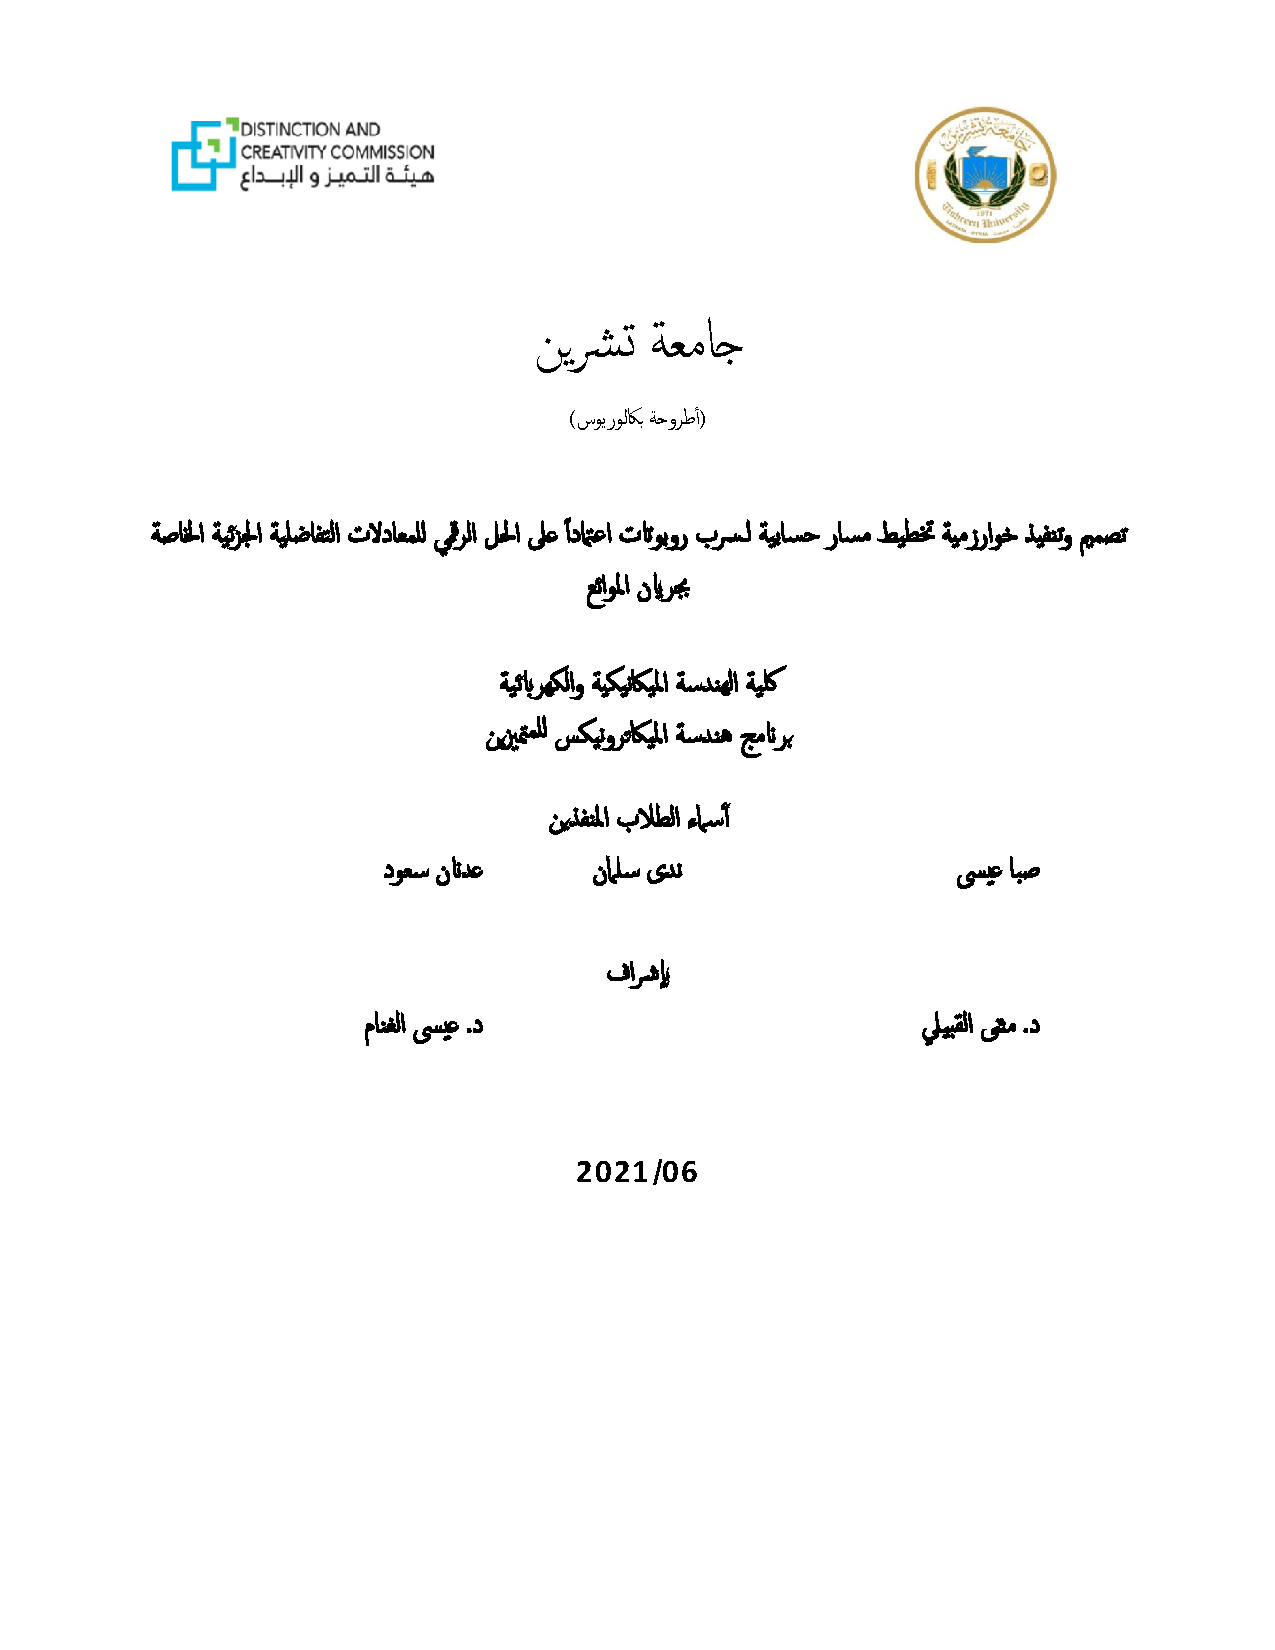
\includepdf[pages=-]{01-cover.pdf}
	
	\begin{english}
		\begin{center}
			\textbf{Abstract}
		\end{center}
		Formation of non-holonomic swarm robots has received a lot of considerations in both academia and industry over last two decades. Many path planning methods produce collision-free paths for a group of multiple robots, but many of them are computationally expensive and complex to implement and develop. In addition, these methods do not find a solution in all environments, or they find a solution that is not optimal. In this project, we present a computational motion planning algorithm based on fluid dynamics PDE for Robotic Swarms.
This proposed method features a computationally cheap algorithm, and it is easy to develop using updated tools and hardware. But, most importantly, it always ensures finding a path, because partial differential equations of fluid dynamics always finds a solution that describes the movement of the fluid’s particles towards a goal. The aforementioned feature gives this algorithm a clear advantage because it is reliable, and it produces a smooth path.
The validity of this algorithm will be tested on a robotic swarm platform that we designed and implemented to ensure high quality and ease of use. The control of the swarm is preformed centrally, and a visual feedback is provided continually to the central computer from a camera that is fixed above the robots.  
	
		\pagebreak
	\end{english}
	
	
	
	\section{موجز البحث}
	
	تعد مضمنات هذا البحث أحد القضايا التي تطرق لها الباحثون بكثرة واهتمام في الفترة الأخيرة: التشكيل السرابي للروبوتات غير الهولنومية.  هناك العديد من الطرق التي قد توصل مجموعة من الروبوتات من منطقة الى أخرى في فضاء العمل بسلام (أحياناً)، لكن عديدها إما تحوي تعقيدات برمجية وبنية خوارزمية ومخطط حالة غاية في التعقيد، أو أنها لا توفر حل في أغلب الأحوال. نحاول في هذا البحث تقديم خوارزمية تخطيط مسار لسرب من الروبوتات الغير هولنومية في بيئة مكتظة باعتبارها تابعة بالحالة للحل الرقمي لمعادلة جريان المائع من منطقة إلى الأخرى بشكله المستقر.
من مزايا الحل المقدم أنه رخيص حسابياً ويمتلك العديد من العناصر القابلة للتسريع باستخدام أدوات حسابية وعتاد حاسوبي جديد، لكن محور البحث يكمن في مكان آخر. نحاول في هذا البحث تقديم طريقة حتمية لإيجاد مسارات حركة هذه الآليات من منطقة لأخرى في فضاء العمل، فالمعادلات الرياضية لجريان السوائل حتماً ستجد حلاً يقوم بإيصال جزيئات المائع من المنطلق للهدف. هذه الحتمية ستعطي أفضلية واضحة للطريقة المقترحة لسببين: موثوقية الطريقة (إذا كان الوصول ممكن فهو حتماً ضمن مجموعة الحل)، ونعومة المسارات المنتجة (مما سيمكن الآليات الغير هولنومية من تقليص الفارق العتادي مع الهولنومية).
سيتم اختبار طريقة الحل المقترحة على منصة روبوتات قمنا بتصميمها وتنفيذها بشكل كامل، مع مراعاة عوامل مثل جودة التصنيع والمرونة والسهولة في الاستخدام والتعديل والتكلفة المناسبة. تم تصميم المنصة بحيث أن يتم التحكم والتواصل مع الروبوتات بواسطة حاسوب مركزي ويتم مراقبتها بواسطة كاميرا مُثبتة أعلى المنصة.

	
	\tableofcontents
	
	
	\chapter{مقدمة البحث}
	
	\section{خلفية وأهداف البحث}
	إنّ مفهوم الأسراب مأخوذ من الطّبيعة، حيث تمّت محاكاة أسلوب التّعاون بين الأسراب البيولوجيّة (النّمل، النّحل، الأسماك..) ونُقل هذا المفهوم إلى الرّوبوتات. يمكننا تصنيف الأسراب البيولوجيّة إلى أسراب أرضيّة وأخرى جويّة، وكذلك الأمر بالنّسبة للرّوبوتات. يختلف هذان النّوعان فيما بينهما من ناحية التّطبيق بشكل أساسي وقد اعتمد البحث \cite{b1} على تصنيف التطبيقات حسب نوع المهمّة الّتي تتولّاها الرّوبوتات (تغطية منطقة ما، مهمّات خطيرة، مهمّات يلعب الوقت فيها دور أساسي...).
يعدّ تخطيط المسار الحسابي للروبوتات الأرضيّة مشكلة مطروقة جداً في الوقت الحالي لما لها من أهمية في توفير الوقت، الطاقة، والعتاد الحسابي. حسابياً، إنّ مشكلة تخطيط المسار الأمثل لأي آلية هي مسألة \textenglish{NP-Hard} \cite{b2,b3}. تتعقد أليات الحساب وتبعاته عند التعامل مع بيئة ديناميكية، أو عند القيام بتخطيط مسار أكثر من كائن في ذات الوقت.
يهدف المشروع الى البحث في إمكانية تطوير آليات لتخطيط المسار الحسابي لمجموعة كائنات اعتماداً على معادلات الجريان النّاتجة عن حل المعادلات التّفاضلية الجزئيّة لحركة الموائع. لقد قدّم كلّ من نافيير وستوكس معادلات كافية لنمذجة حركة السائل في الظروف المُختلفة، وسيتمّ الاعتماد عليها في إنشاء المسارات.

	\section{الدراسات المرجعية}
	يقدم هذا القسم مجمل ما تم مراجعته بهدف تصميم وتنفيذ خوارزمية البحث والمنصّة الفعالة.

\subsection{التصنيف والتصميم}

إنّ الأنظمة متعدّدة الروبوتات تلاقي اهتماماً كبيراً في المراجع ولاسيّما في الآونة الأخيرة؛ نظراً إلى أنّ مجالات التّطبيق والمهام الّتي تواجهها تزداد تعقيداً. لقد تمّ اقتراح تصنيف جديد في عام 2004 اعتماداً على ثلاث نقاط أساسيّة: (1) عقلانيّة التّصميم، (2) الوظائف التّقنيّة الاساسيّة (لكّل من العتاد الصّلب والبرمجيّات)، (3) المهمّات الّتي يجب أن تقوم الرّوبوتات بتنفيذها. حيث تمّ التّصنيف على عدّة مستويات ضمن فئتين أساسيّين: الأبعاد التنسيقيّة، وأبعاد النّظام كما هو موضّح في الجدول \ref{06:table:1} \cite{b4}. 

\begin{table}[]
	\begin{tabular}{|l|l|}
		\hline
		الأبعاد التّنسيقيّة Coordination Dimensions & أبعاد النّظام System Dimensions       \\ \hline
		التّعاون   Cooperative                      & الاتّصال   Communication              \\ \hline
		المعرفة Knowledge                           & تكوين   الفريق team Composition       \\ \hline
		التّنسيق   Coordination                     & هيكليّة   النّظام System Architecture \\ \hline
		التّنظيم Organization                       & حجم الفريق Team Size                  \\ \hline
	\end{tabular}
\caption{الأبعاد التنسيقية وأبعاد النظام}
\label{06:table:1}
\end{table}

وفي العام التّالي طرحت الورقة البحثيّة \cite{b5} تبين أنّ أي فعل يقوم به أي روبوت يَأخذ بالحسبان الأفعال الّتي تقوم بها بقيّة الرّوبوتات، وهكذا ينتج مجموعة من الرّوبوتات الّتي تعمل باتّساق لتحقيق أفضل أداء ممكن. وقد أظهرت هذه الآليّة من التّنسيق أداء عالٍ؛ حيث تمكّنت الروبوتات من اكتشاف بيئتها في وقت أقل مقارنةً مع المنهجيّات الأخرى الّتي لا تعتمد على التنسيق بين الرّوبوتات بشكل صريح. وبالرّغم من النّتائج الجيّدة الّذي حقّقها النّهج المتّبع في البحث \cite{b5}، إلّا أنّ هناك بعض النقاط الّتي تحتاج إلى تطوير، حيث يجب مناقشة الحالات الّتي يتمّ فيها تعطّل أحد الرّوبوتات أو حدوث تغيّر ما في البيئة المحيطة بها.

ومن ناحية أخرى، نالت أعداد الرّوبوتات الّتي تشكّل السّرب اهتماماً كبيراً في مجال البحث العلميّ. على الرّغم من أنّ سلوك كلّ روبوت على حدا يُعدّ سلوكاً بسيطاً، إلاّ أنّه عندما تعمل هذه الرّوبوتات معاً يصبح سلوكها أكثر تعقيداً. أشار \cite{b6} إلى أنّ فهم الرّوبوتات بشكل فرديّ هو أمرٌ سهل، أمّا بالنّسبة لتوقّع سلوكها معاً فهو أمرٌ صعب المنال. لقد تمّ عرض النّهج المعتمد من قبل \cite{b6} من خلال التّحليل العميق لخوارزميّة السّرب المُتّبعة والنّموذج الاحتمالي المُرتبط بها؛ حيث تمّ فحص خوارزميّة التّحكم باستخدام فضاء الحالة المُطوّرة من قبل \cite{b7} على مجموعة من الرّوبوتات الباحثة عن طعام.


 لقد قام \cite{b6} باستخدام خوارزميّة ألفا في شبكة الاتّصال اعتماداً على المنطق الزّمني $ (Temporal logic) $، حيث تمّ التّركيز على حالة الرّوبوتات بدلاً من الموقع وتفاصيل حركة كلّ روبوت. ولكنّ وبالرّغم من النّتائج المُرضية وصل اليها البحث، إلا أنه لم يتمكّن من إجراء عملية التّحليل سوى على عدد قليل من الرّوبوتات بسبب مشكلة انفجار الحالة $ (state explosion) $ التي ظهرت أثناء عمليّة فحص النّموذج الرّياضي. 
 
 \subsection{تخطيط المسار}
 
 تُعدّ مشكلة تخطيط المسار متعدد الروبوتات مشكلة معقدة حسابياّ لأنّ صعوبة الحساب تنمو مع عدد الروبوتات. إنّ وجود قيود وعوائق في المسار يولّد مشكلة كبيرة، ومن هنا بدأت عمليّة البحث عن خوارزميّات لحلّ هذه المشكلة. أحد الخوارزميّات المُتّبعة لحلّ مشكلة المسار المقيّد هي الـ \textenglish{Visibility Graph (VG)}. تبدأ هذه الطريقة بتشكيل الرّسم البياني عن طريق رسم العقد (Nodes) والحواف (Edges) باستخدام تقنيّة التّصوير بالأشعّة، ومن ثمّ تحديد البيان الموجّه. يتمّ بعد ذلك إيجاد المسار الأقصر باستخدام خوارزميّات إيجاد الطريق الأقصر في البيان. نذكر هنا أن المسار النّاتج عادةً قريب جدّاً من العوائق.
 
 وكان البحث \cite{b8} قد قدّم عام 1985 طريقة فريدة لتفادي العوائق اعتماداً على تقنيّة الـ $ (Potential Field) $، حيثُ تمّ التّحكم بالروبوتات على عدّة مستويات وبالزّمن الحقيقي. وتتميّز هذه الطريقة بإمكانيّة توسيع الحلّ ليشمل البيئات ذات العوائق المُتحرّكة باستخدام حقل كموني متغيّر مع الزّمن.  وفي عام 2006 قدّم العمل \cite{b9} طريقة حقل كموني لتخطيط مسار الروبوت بالاعتماد على ناتج جمع تابعين هما: تابع $ (repulsive) $ الذي يتجنب المسارات القريبة من العوائق، وتابع $  (Attractive) $ قيمته تتعلق بالمسافة عن الهدف.
 
 إنّ طريقة الـ $ potential field $ هي طريقة مباشرة لحساب الحقل المتجهات $ (vector field) $ اعتماداً على موقع الهدف والعوائق، ولكنها تتطلّب روبوتات مُتحكّم بها بشكل كامل (قادرة على التّحرك بأي اتّجاه بشكل آني). على خلاف الحقل الكموني، طرق تخطيط المسار المعتمدة على الدّوال التّدفقيّة $ Stream function $ لا تتطلب التّحكم ذلك، كما أنّها تضمن تحوّل جميع نقاط التّوازن إلى نقاط سرجيّة، مما يعني ضمان وصول الروبوت إلى هدفه. لقد أظهرت عمليّة تخطيط المسار المُعتمدة على الدّوال التّدفقيّة المطروحة في \cite{b10} فعاليّة وسرعة عاليّة في التّكيف مع التّغيرات في الشّروط. على عكس طرق تخطيط المسار الأخرى، الطّرق الّتي تعتمد على الدّوال تتميز بمظهرها الحدسيّ بالنّسبة لمراقب الخارجي. إنّ وجود أكثر من حاجز لا يضمن دائماً الحصول على نتائج صحيحة، لكن هذا المثال يوضّح أن السلوك لا يزال مقبولاً كما هو موضح في الشكل \ref{06:fig:1}.
 \begin{figure}[h]
 	\centering
 	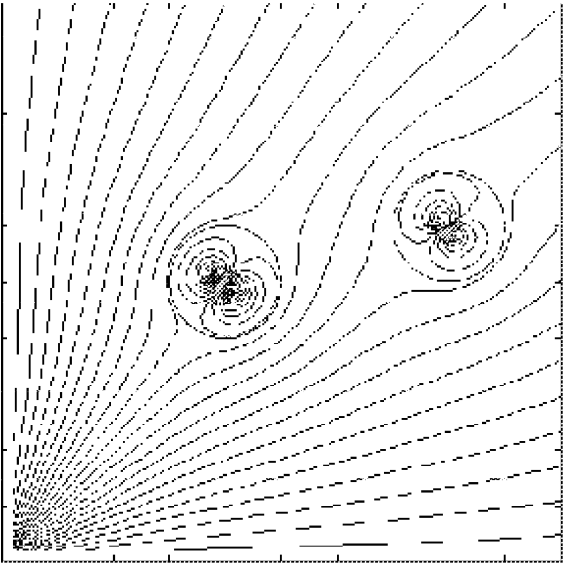
\includegraphics[width=0.5\linewidth]{figs/06/fig1}
 	\caption{مثال على الدوال التدفقية}
 	\label{06:fig:1}
 \end{figure}


في عام 2015 تمّ طرح سلالات فورونوي \textenglish{VORONOI STRAINS} كخوارزميّة جديدة لتخطيط المسار والّتي حقّقت فائدة مهمّة على صعيد البيئات المعقّدة \cite{b9}. لقد حقّقت هذه الخوارزميّة نتائج مثيرة للاهتمام في مساحات عمل فيها عدد كبير من العوائق، فقد أظهرت حلولاً أفضل بكثير من خوارزميّة PSO البسيطة والمُطوّرة من أجل نفس عدد التّكرارات. إضافة إلى ذلك، أثبتت أنّها أكثر صلادة وأقل اعتماديّة على الحالة الابتدائيّة (العشوائية). كما تتميّز هذه الخوارزميّة باحتماليّة أكبر لتجنّب النّقاط الصّغرى المحليّة، ولكن قد أثبتت التّجارب أن عمليّة االأمثلة هذه غير مُجدية مالم تكن البيئة معقّدة بشكل كافِ.

أثناء تخطيط الحركة يمكننا تصنيف العمل إلى صنفين أساسيّن؛ فإمّا أن يتمّ تخطيط المسار بشكل كامل قبل البدء بالحركة (offline)، أو أن تتمّ عمليّة التّخطيط بشكل تدريجي أثناء الحركة (online).

 
  في \cite{b11} ، تم التّركيز على تخطيط المسار بشكل كامل قبل بدء الحركة، بالإضافة إلى وجود حواجز ثابتة، وهي إحدى الأمور الّتي أعطت هذا البحث محدوديّته. تتميّز طريقة تخطيط المسار المُقترحة في \cite{b11} بأنّها تمكّننا من الحصول على مسار ثلاثي الأبعاد مثالي يمكن الروبوتات من التحليق على ارتفاعات منخفضة في بيئة ذات تضاريس مُعقّدة.
  
  وفي عام 2020 طُرحت الورقة البحثيّة \cite{b12} بهدف توجيه روبوتات طائرة في مجال جوّي مفتوح وتضاريس غير معلومة لتتفوق بذلك على البحث \cite{b11} وذلك عبر حلّ معادلة الاستمراريّة للموائع. لقد حقّقت هذه الدّراسة وقتاً أقلّ من أربع طُرق أخرى $( A*, Dijkstra, DP, PE) $.
  
  إضافة إلى الخوارزميات التقليدية، العديد من الدراسات أظهرت نتائج خوارزميات التعلم الآلي لحل هذه النوع من المشكلات. في \cite{c1} تم استخدام الشبكات العصبونية الالتفافية لتحسين حلول الخوارزميات التقليدية كما نجد في \cite{c2} أنه تم استخدام خوازرمية تعلم Q-learning معتمدة على الخوارزمية المحسنة \textenglish{improved particle swarm optimization}. تهدف الخوارزميات المستخدمة الى تقليل طول المسار وزمن الوصول وزوايا دوران الروبوتات لتقليل استهلاك الطاقة. تمت المقارنة بين اربع خوارزميات وايجاد النتائج باختلاف عدد الروبوتات في السرب هي CQL و PSO وIPSO-DV  و QIPSO-DV وأظهرت النتائج تفوق QIPSO-DV على باقي الخوارزميات كما يمكن ملاحظة تراجع أداء هذه الخوارزمية مع زيادة عدد الروبوتات ولاسيما من حيث زمن التنفيذ وعدد التكرارات اللازمة للوصول الى الحل الأمثل (إن وجد) .
  في \cite{c3} تم اقتراح تقسيم الخريطة الكلية الى خرائط بيان جزئية sub-graphs مع قيود على الدخول والخروج من كل خريطة وذلك لضمان إيجاد المسار. بعد التجريب، تم التوصل الى حل فعال وسريع نسبيا لكنه لا يضمن ايجاد مسار أمثل وبحاجة إلى عمليات معالجة لاحقة لتقليل المسافات الضائعة.  
  
   يعد موضوع انشاء طريق باستخدام الحل الرقمي للمعادلات التفاضلية الجزئية موضوع حديث عالمياً ويحتاج الكثير من العمل، قدمت واحدة من الأبحاث القائمة على موضوع استغلال جريان السوائل في توليد المسار عام 2017، حيث تهدف \cite{b13} الى انشاء المسار الأفضل لحركة سفينة باستخدام طريقة $ lattice Boltzmann $ الرقمية. البحث لم يناقش آلية انشاء طريق من نقطة إلى اخرى في فضاء العمل، بل ناقش عبور منطقة تحتوي عوائق بشكل عام. إضافة لذلك، فإن الحل الرقمي باستخدام $ lattice Boltzmann $ لم ينتج حقول متجهات سرعة تحمل نفس السلوك الفيزيائي للسوائل، يمكن التحقق من ذلك بالنظر في سلوك الحقل عند الحواجز في الشكل \ref{06:fig:2}.
   
         
   \begin{figure}[htbp]
   	\centering
   	\includesvg[width=0.85\linewidth]{figs/06/fig06_2}
   	\caption{التدفق المولد باستخدام الخوارزمية $ lattice Boltzman $. يمكن ملاحظة السلوك غير الفيزيائي للسائل بالنظر الى تداخل السائل مع الجدران.}
   	\label{06:fig:2}
   \end{figure}
   
   
      
      وكان قد طُرح في عام 2009 نظام  قوي وسريع لتخطيط المسار للملاحة الآليّة \cite{b14}، والفكرة الأساسيّة الّتي اعتمد عليها هذا البحث هي انشاء المسار عبر نشر موجتين متتاليتين، كما في الشكل \ref{06:fig:3}. تبدأ بموجة أولى تكون ذات سرعة قليلة نسبيّاً تُمكّن الرّوبوت من نقل طوبولوجيا الخريطة إلى الحاسوب، بينما تنتقل الموجة الثّانية ذات السّرعة العالية في الخريطة وذلك من أجل تكوين مسار من نقاط جهات الانتشار ذات التّقعّر الأعلى. وفي النّهاية يمكن التّحكم في المسارات المثلى المخطّطة اعتماداً على معامل واحد: المسار الأقصر، الأكثر أماناً، أو الهجين.
       \begin{figure}[h]
      	\centering
      	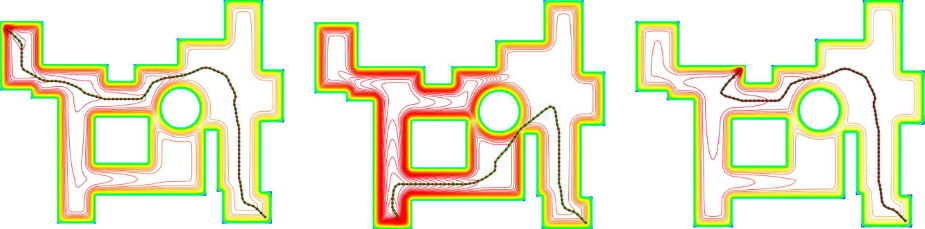
\includegraphics[width=0.9\linewidth]{figs/06/fig06_3}
      	\caption{الأمواج المتقدمة والمتأخرة في العمل\cite{b14}}
      	\label{06:fig:3}
      \end{figure}
      
      
      \subsection{الاتصال}
      
      كما أشرنا سابقاً، فإنّ فكرة الاسراب مأخوذة من الأسراب البيولوجيّة، حيث أن أساس التّحكم في سلوك هذه الأسراب هو تبادل المعلومات. يتمكّن الأفراد في الاسراب البيولوجيّة من تبادل المعلومات بشكل مباشر عن طريق المجسّات، الحركة، أو الصّوت. استوحى \cite{b15} تصنيف أسراب الرّوبوتات من الاسراب البيولوجيّة، حيث تمّ التّصنيف إلى مجموعتين أساسيّتين:
            
      \begin{itemize}
      	\item \textbf{أولاً: التّفاعل عن طريق التّحسس:} هو الطّريقة الأبسط للتّواصل بين الرّوبوتات. تتطلّب من الرّوبوت التّمييز بين الأقران والبيئة المحيطة به. يطلق على هذا النّوع من الاتّصال بالصّريح. 
      	\item \textbf{ثانياً: التّفاعل عن طريق البيئة:} حيث تستخدم الرّوبوتات البيئة كوسيلة للتّواصل فيما بينها. يسمّى هذا النّوع بالتّواصل الضّمني. أسراب النّمل مثال شهير على الاتّصال الضّمني؛ حيث يتواصل أفراد السّرب عن طريق إفراز وتتبع مادّة الفيرومون \cite{b15}.
      \end{itemize}
      
      هناك العديد من طرق الاتّصال المستخدمة في أسراب الروبوتات، ومن التّقنيات المستخدمة للاتصال بين الرّوبوتات في السّرب الواحد (الأشعة تحت الحمراء، البلوتوث، الـWi-Fi، ZigBee، ...). تعد عمليّة اختيار التّقنيّة المناسبة مهمّة جدّاً لأنها مؤثر مباشر على أداء السرب، لذلك تتمّ بناءً على عدّة معايير (البيئة الّتي تعمل بها الرّوبوتات، مدى الاّتصال، معدّل نقل البيانات، ...) وقد قام العمل \cite{b16} بمقارنة أداء هذه الطّرق.
      
وعندما نتوجّه نحو الاتّصال اللاسلكي فإنّ شرائح الـ ESP8266 توفر ما يجعلها الخيار الأمثل، فهي منخفضة التّكلفة مقارنة بأدائها، وتدعم بروتوكولات TCP/IP بشكل كامل.  تتكون من SoC يحوي معالج Xtensa Tensilica [32bit]  وشريحة Wi-Fi تدعم بروتوكول  الاتّصال اللاسلكي IEEE 802.11b/g/n،  اضافة إلى العديد من الميّزات كما ورد في مقدّمة \cite{b17}.

مجتمع الـ Opensource الخاص بشريحة الـ ESP وفّر مكتبة PainlessMesh المبنية خصّيصاً لتشكيل شبكات تعتمد على أجهزةESP8266؛ حيث أنّها تبني شبكة خالية من الحلقات وتقوم بالتّحديث كلّ 3 ثواني. إلّا أنّه ومع الأسف كان هنالك انخفاض ملحوظ في أداء الشّبكة مع ازدياد العقد المُتّصلة بها كما كان واضحاً في نتائج التّجارب الّتي قام بها \cite{b17}.


بصورة عامة، تكمن الغاية الأساسية من تصنيع وتركيب الروبوتات بشكل عامة في الوظيفة التي ستقوم بها على أرض الواقع، ومن هنا يصبح للتنفيذ الفعلي أهمية كبيرة حيث أن محاكاة أداء الروبوتات ومهما كان دقيقا، فإنه يستخدم فقط لتقييم التصميم قبل التنفيذ الفعلي.
عالمياً، نجد تنوع كبير في منصات أسراب الروبوت وفق الغاية منها، بعضها تكون لأهداف تعليمية والبعض الآخر لأهداف بحثية لختبار صحة الخوارزميات كما في بحثنا هذا. تقدم \cite{c4} مراجعة عامة لأهم وأشهر منصات أسراب الروبوت ومقارنة من حيث الخصائص العامة والحجم والسعر والحساسات المستخدمة. تم التوصل إلى أن معظم هذه المنصات مناسبة جدا للأغراض البحثية، كما أن بعض المنصات مثل MarXbot وsbot وPheeno مناسبة للاستخدام على أرض الواقع وذلك لمرونة التصميم وإمكانية عبورها ضمن البيئات الصعبة. نجد في الجدول ملخصاّ عن المقارنة بين المنصات.

\begin{table}[]
	\begin{tabular}{@{}lp{10pt}p{10pt}p{10pt}r@{}}
		\toprule
		& التكلفة (دولار)          & الحجم (سم)               & عمر البطارية (ساعة)   & \multicolumn{1}{c}{الخصائص المميزة}                                                     \\ \midrule
		Colias \cite{c5}   & 25                      & 4                        & 4                     & وحدة استشعار بالأشعة تحت الحمراء ذات مدى   طويل                                         \\
		AmiR \cite{c5}    & 65                      & 6.5                      & 2                     & حساسات ذات درجة حساسية عالية                                                            \\
		Kilobot \cite{c6}  & 14                      & 3.3                      & 3                  & دواليب ذات حركة بنمط Omni                                                               \\
		R-one \cite{c7}     & 220                     & 10                       & 6                     & قابلة للتغير بشكل ذاتي، آلية اقتران                                                     \\
		s-bot \cite{c8}    & -                       & 15                       & 1                     & آلية اقتران، قابلية تجمع بشكل ذاتي،   كاميرا متحركة بكل الاتجاهات                       \\
		e-puck \cite{c9}    & 1200                    & 75                       & 2                     & يمكن محاكاتها باستخدام محاكي WEMBOTS و ENKI                                             \\
		MarxBot \cite{c10}  & -                       & 17                       & 8                     & قابلة للتغير بشكل ذاتي، آلية اقتران،   كاميرا متحركة بكل الاتجاهات، تصميم ببنية معيارية \\
		Pheeno \cite{c11}   & \multicolumn{1}{l}{270} & \multicolumn{1}{l}{12.7} & \multicolumn{1}{l}{-} & آلية قبض، كاميرا                                                                        \\ \bottomrule
	\end{tabular}
\end{table}
	
	\section{أهداف المشروع}
	\begin{itemize}
	\item تصميم وتنفيذ روبوتات صغيرة الحجم وعالية الجودة وسهلة الاستخدام.
	\item تصميم منصة عمل مناسبة تمكننا من اختبار أي خورازمية تخطيط مسار ضمن بيئة عمل معروفة سابقاّ.
	\item تطوير وبرمجة خوارزمية تخطيط حسابي تعتمد على المعادلات التفاضلية الجزئية لروبوت واحد ولسرب من الربوتات.
	\item  برمجة خوارزميات شهيرة أخرى في تخطيط مسار الروبوت لروبوت واحد ولسرب من الروبوتات.
	\item استخلاص نتائح تؤكد صحة الخوارزمية المقترحة وتفوقها على الخوازميات التقليدية وغير التقليدية من ناحية حتمية إيجاد المسار وعوامل أخرى.
\end{itemize}
	
	\section{مخطط العمل}
	يوضح المخطط التالي آلية كاملة لعمل المشروع. نبدأ من عرض البينة البرمحية الموجودة على الحاسوب المركزي والتي تتكون من نظام تشغيل روس مكون من ثلاثة عقد تتصل مع بعضها بتقنية \textenglish{Publish / Subscribe}، ثم نوضح تواصل هذه النظام مع مخدم بروتوكول MQTT المسؤول عن تحقيق التواصل مع الروبوتات حيث تشترك الربوتات بـ topic التي تحوي الرسائل الحاملة لنقاط المسار. بالنسبة للنظام البرمجي الموجود على كل من الروبوتات، تستقبل شريحة الاتصال الرسالة من المخدم وتنقلها إلى المعالج ليثيوم باتباعها وفق خوارزمية التصحيح. أنظر الشكل \ref{fig:08-graph}.


\begin{figure}
	\centering
	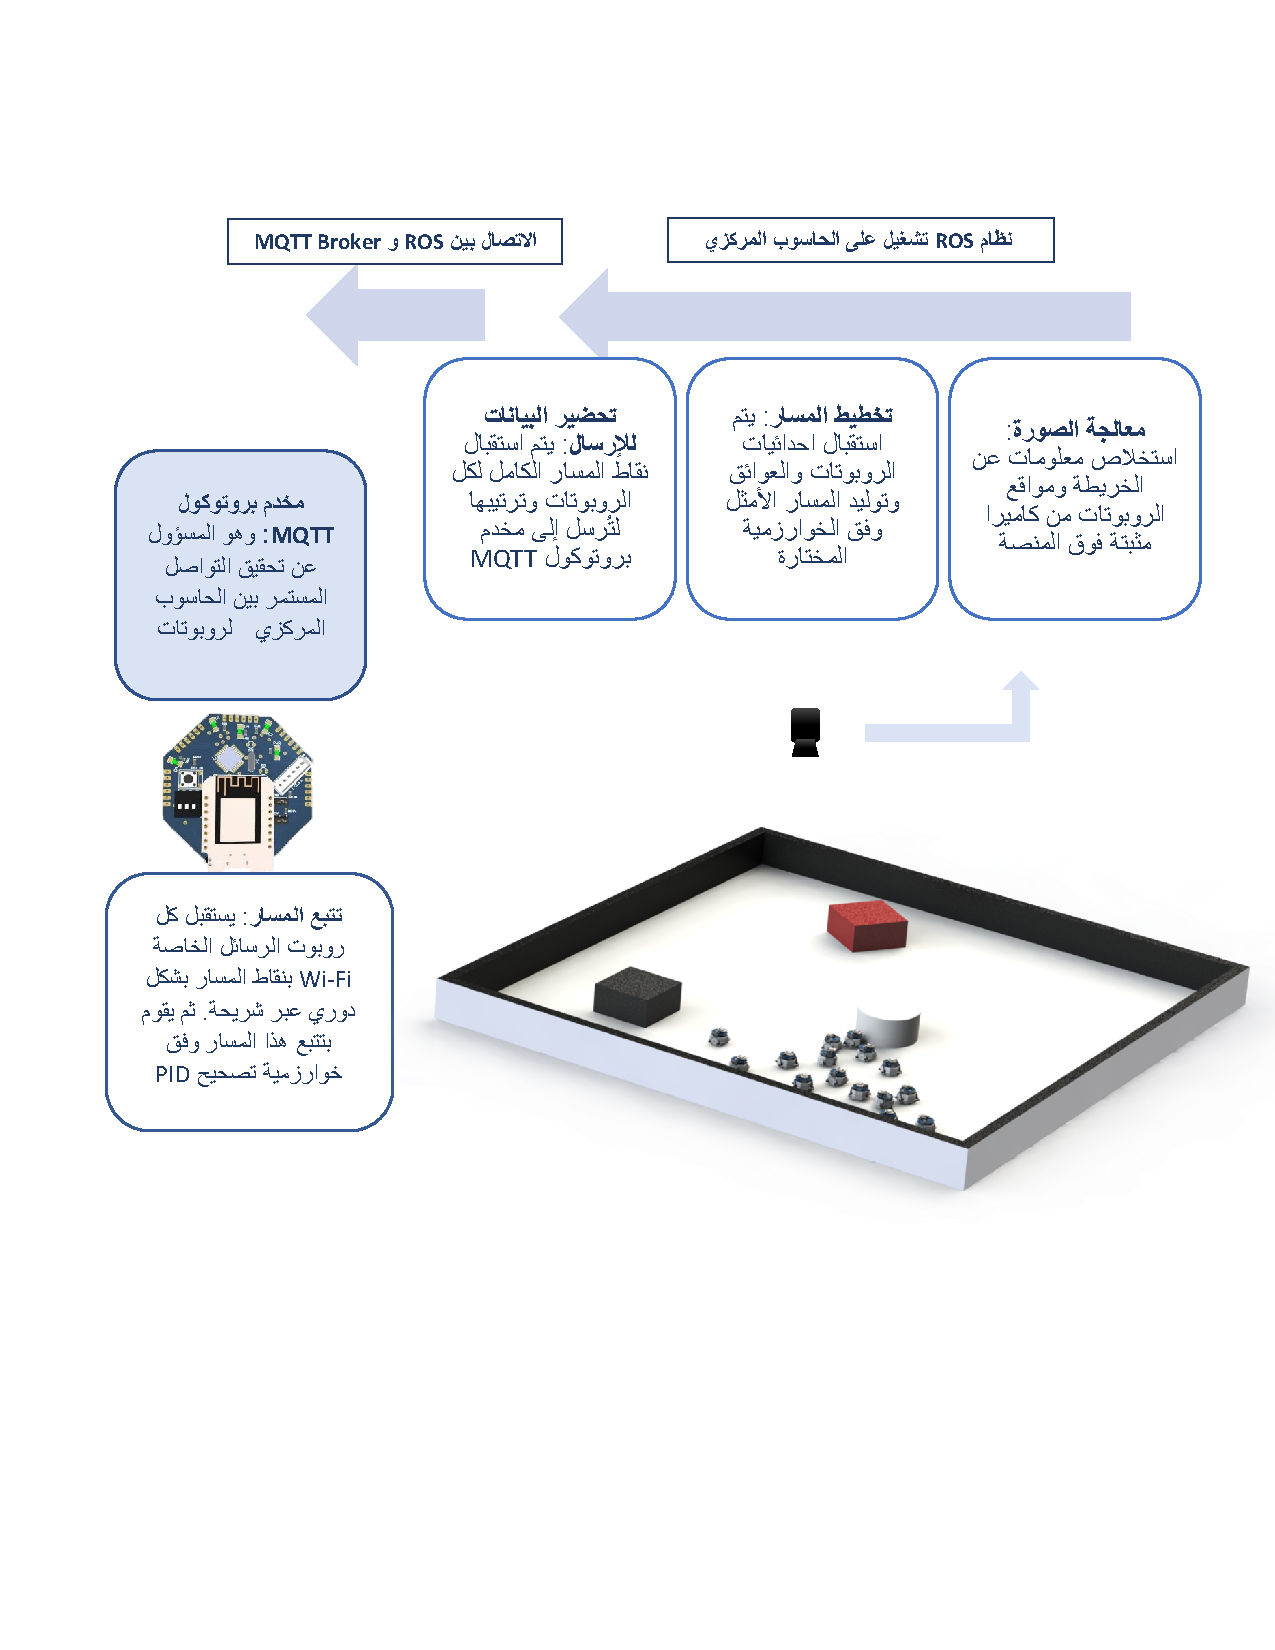
\includegraphics[width=0.95\linewidth]{08-graph}
	\caption{}
	\label{fig:08-graph}
\end{figure}

	
	\section{مخطط الأطروحة}
	بعد أن قدمنا معلومات عن خلفية البحث والدراسات المرجعية وعرضنا مخططاً يوضح آلية عمل المشروع بكامل أجزائه،  ننتقل إلى الفصل الثاني لشرح الدراسات النظرية والنمذجة والمعادلات الرياضية المستخدمة وذلك بما يتضمن خوارزميات تخطيط المسار ونظام الاتصال بشكل أساسي. نفدم في الفصل الثالث المعلومات الكاملة عن عملية تصنيع الروبوتات بما في ذلك اختيار القطع الكهربائية والالكترونية وتصنيع الدارات وطباعة الأجسام كما نذكر شرحاً تفصيلياً عن نظام العمل البرمجي المُطور لتشغيل الروبوتات والحاسوب المركزي. في الفصل الرابع نقدم شرحاً عن النتائج التي توصلنا إليها حتى الآن.
	
	
	\chapter{الدراسة الرياضية والنمذجة}
	
	
	\section{تخطيط المسار لروبوت واحد باستخدام الطرق التقليدية}
	
	
\subsection{الخوارزميات المعتمدة على البيان}

تعتمد هذه الخوارزمية على فضاء العمل لإنشاء بيان يمثل كل الأماكن المتاحة في فضاء العمل متضمناً نقطتي البداية والنهاية. يضمن هذا التمثيل ترميز وجود كل الطرق المتاحة وكذلك يضمن آلية لتفادي العوائق عن طريق حذف عقدها من البيان. بعد الانتهاء من التقطيع نعبر البيان من نقطة البداية الى النهاية باستخدام احدى خوارزميات عبور البيان الشهيرة $ (A^*, Disjkstra)$. يمثل الشكل \ref{fig:fig101} طريقة نقل فضاء العمل الى البيان.

\begin{figure}
	\centering
	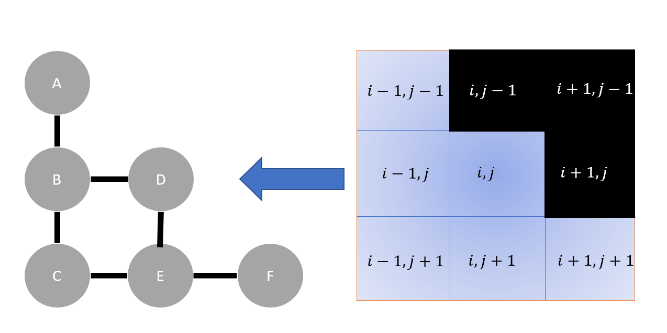
\includegraphics[width=0.8\linewidth]{figs/10/fig10_1}
	\caption{ تحويل فضاء العمل المقطع إلى بيان غير موجه}
	\label{fig:fig101}
\end{figure}

\subsubsection{المسار باستخدام A*}

خوارزمية عبور بيان وانشاء مسار تستخدم في كثير من مجالات علم الحاسوب نظرً لكمالها، مثاليتها، وكفاءتها. في الأنظمة التي من الممكن حساب الطريق بشكل استباقي، يمكن تجاوز أدائها من قبل الخوارزميات التي تستطيع حساب المسار قبل البدء بالتنفيذ \cite{d1} . واحدة من أكبر مشاكلها هي تعقيدها المكاني:$  O\left(b^d\right) $.

\subsubsection{المسار باستخدام Dijkstra}

هي خوارزمية صممت لإيجاد المسار الأقصر بين عقدتين في بيان معين. تعتمد الخوارزمية على إيجاد الطريق من خلال عبور عقد البيان بالتدريج ثم حساب معاملات المسافة وإيقاف البحث في حال مواجهة عائق \cite{d2}


\begin{table}
	\centering
	\begin{tabular}{cc}
		
		\begin{subfigure}{0.4\textwidth}
			\centering
			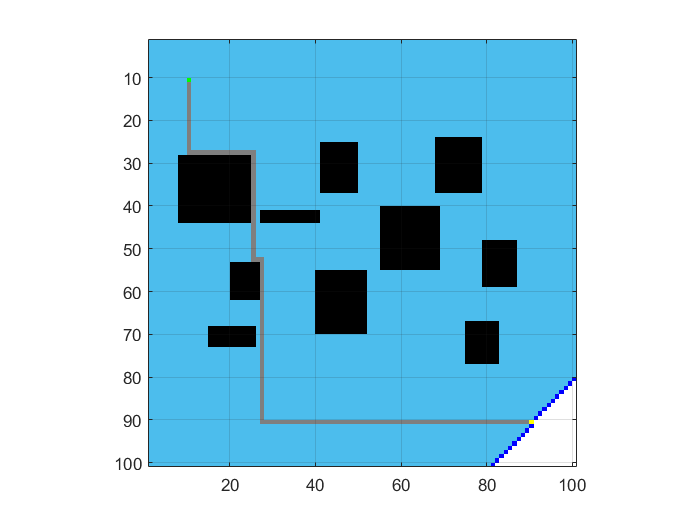
\includegraphics[width=0.9\linewidth]{figs/10/fig10_2}
		\end{subfigure}&
	
		\begin{subfigure}{0.4\textwidth}
			\centering
			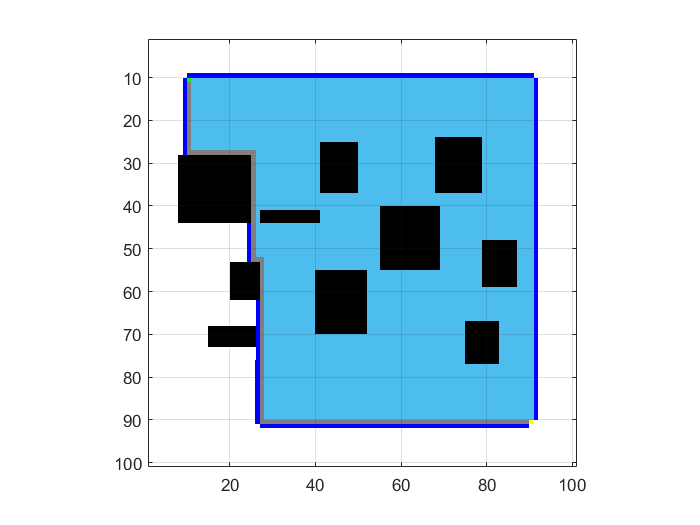
\includegraphics[width=0.9\linewidth]{figs/10/fig10_3}
		\end{subfigure}
	\end{tabular}
	\caption{خرائط لحل كل من خوارزميتي البيان.}
	\label{10:fig:graph}
\end{table}

\subsection{خوارزمية الحقل الكموني}
تعتمد خوارزمية \textenglish{potential field} على بناء خريطة افتراضية يتحرك الروبوت وفقها اعتماداً على مواقع المبدأ والهدف والحواجز. يمكن أن يتم حساب المسار اعتماداً على خريطة حواجز معروفة مسبقاً أو بالزمن الحقيقي اعتماداً على حساسات مثبتة على الروبوت أو على الحلبة. تم عرض هذه الخوارزمية لأول مرة عام 1985 \cite{b8} حيث قدم البحث الحقول $ potential field $ كجزئين، جزء جاذب وجزء منفر. الجزء الجاذب يقوم بسحب الروبوت نحو الهدف، أما الجزء المنفر يقوم بإبعاد الروبوت عن العوائق بمسافة أمان تحدد مسبقا. 

تستخدم هذه الخوارزمية بكثرة في تطبيقات تخطيط المسار وذلك لبساطتها وسهولة تطبيقها ولا سيما أنها تعطي نتائج جيدة في البيئات البسيطة التقليدية، لكن يوجد عدة سلبيات مرتبطة باستخدام هذه الخوارزمية.
أحد السلبيات هي أن الروبوت يمكن أن يحتجز في قيمة صغرى محلية مما يؤدي الى توقفه عن الحركة نهائيا وعدم وصوله الى الهدف. تم تطوير العديد من الطرق لحل هذه المشكلة متل تتبع الحائط   \cite{d4}  وإضافة حواجز افتراضية \cite{d5}. من السلبيات الأخرى هي عدم قدرة الروبوت على المرور بين حواجز متقاربة. عند عبور الروبوت بممر ضيق يقوم بحركة اهتزازية غير مستقرة نتيجة تأثره بقوى الحقل المنفر \cite{d6}.


\textbf{توليد المسار وفق $ potential field $:}

شعاع الحقل الجاذب يحسب من موقع الروبوت الى الهدف، أما شعاع الحقل المنفر يكون من موقع الحاجز الى موقع الروبوت. بجمع الشعاعين نحصل على شعاع يحدد اتجاهه اتجاه حركة الروبوت، ومطاله سرعة الروبوت. ليكن $ (x_r,y_r) $ موقع الربوت الابتدائي و $ (x_g,y_g) $ موقع الهدف و $ (x_o,\ y_o)   $ موقع الحاجز في خريطة ثنائية الأبعاد.

يعطى شعاع الحقل الجاذب بالعلاقات التالية:

\begin{equation}
{\vec{v}}_{attr}=\left(\begin{matrix}x_{atrr}\\y_{atrr}\\\end{matrix}  \right)
\end{equation}

\begin{equation}
\left(\begin{matrix}x_{atrr}\\y_{atrr}\\\end{matrix}  \right)=\left(\begin{matrix}x_{g} - x_{r}\\y_{g} - y{r}\\\end{matrix}  \right)
\end{equation}

تعطى المسافة والزاوية بين الروبوت والهدف بالعلاقات التالية:

\begin{equation}
d_o=\sqrt{\left(x_r-x_o\right)^2+\left(y_r-y_o\right)^2}
\end{equation}

\begin{equation}
\theta = tan^-1(\frac{y_r - y_o}{x_r - x_o})
\end{equation}

وبالتالي يعطى شعاع الحقل المنفر بالعلاقات التالية:

\begin{equation}
{\vec{v}}_{rep}=\ (\begin{matrix}x_{rep}\\y_{rep}\\\end{matrix})\ 
\end{equation}

\begin{equation}
x_{rep}=\frac{1}{d_o} cos(\theta), if d_o < s
x_red = 0 , otherwise  
\end{equation}

\begin{equation}
y_{rep}=\frac{1}{d_o} sin(\theta_o), if d_o < s
y_red = 0 , otherwise  
\end{equation}


حيث $ s $ هي قطر المنطقة الفعالية المحيطة بمركز الحاجز.
بجمع شعاعي الحركة الجاذب والمنفر نحصل على شعاع الحركة النهائي:

\begin{equation}
v_{final}^\rightarrow=v_{attr}^\rightarrow+v_{rep}^\rightarrow
\end{equation}

\begin{table}
	\centering
	\begin{tabular}{cc}
		
		\begin{subfigure}{0.35\textwidth}
			\centering
			\includesvg[width=0.9\linewidth]{figs/10/fig10_4}
		\end{subfigure}&
		
		\begin{subfigure}{0.35\textwidth}
			\centering
			\includesvg[width=0.9\linewidth]{figs/10/fig10_5}
		\end{subfigure}
	\end{tabular}
	\caption{عملية حساب المسار في طريقة الحقل الكموني}
	\label{10:fig:pf}
\end{table}



	
	\section{تعميم الحل للأسراب}
	
	يمكن تصور تعميم الخوارزميات السابقة لسرب من الروبوتات بشكل مبسط بالشكل الآتي: نقوم بحساب المسار الأمثل لكل روبوت على حدى باعتبار كل بقية الروبوتات على أنها عوائق، وإعادة توليد هذه المسار بشكل مستمر باستخدام التغذية الراجعة من الكاميرا، ولكن وبسبب طبيعة هذه عمل هذه الخوارزميات لا يمكن تطبيق هذا المفهوم البسيط على أرض الواقع. فكما نجد في \cite{d7} عند استخدام خوارزمية A* لتوليد مسار لسرب من الروبوتات، تطلب التطبيق عدة عمليات معالجة لاحقة وتنظيم لحركة الروبوتات لمنع التصادم، كما تمت الحاجة لتصميم وحل مسألة برمجة خطية لتقليل طول المسار وزمن الوصول.
بالحالة العامة وفي معظم مسائل تخطيط المسار لسرب روبوتات، الهدف هو إيصال كل روبوت من نقطة البداية إلى نقطة الهدف بدون حدوث أي تصادم. كما وجدنا في الدراسة السابقة، فإن الكثير من الدراسات السابقة تعتمد تحسينات على خوارزميات تخطيط المسار التقليدية. في \cite{d7} تم تقدم تقديم خوارزمية جديدة تسمي البحث المعتمد على التصادم\textenglish{ Conflict Based Search (CBS)} وهي طريقة مثلى تتكون من مرحلتين ،مرحلة عالية المستوى ومرحلة منخفصة المستوى. في المرحلة المرتفعة المستوى، يتم البحث في ما يسمى شجرة التصادم\textenglish{ Conflict Tree(CT)} وهي شجرة تُبنى بناء على التصادك بين الروبوتات والعوائق، كل عقدة في الشجرة تمثل مجموعة قيود على حركة الروبوتات. في المرحلة المنخفضة المستوى، تتم عملية بحيث سريع بما يحقق القيود المطروحة في الطبقة العالية المستوى. في معظم الحالات تحقق هذه الخوارزمية مسحاً لعدد أقل من العقد بالمقارنة مع A* وتحافظ في نفس الوقت على الأمثلية.


\subsection{تعريف مسألة CBS}

نعرف كل قيد على أنه ثلاثية بالشكل $ (a_i,\ v,\ t) $ حيث أن الروبوت $ a_i $ ممنوع من المرور بالعقدة v في الزمن t، خلال إيجاد الحل سيتم ربط كل روبوت بعدد من القيود ولاحقا يجب إيحاد مسار لكل روبوت بحيث يحقق كل قيوده
تعرف التصادم على أنه رباعية بالشكل $ (a_i,a_jو v,t) $ مما يدل على أن الروبوتات $ a_i $ و  $ a_j $ تشغل نفس العقدة v في الزمن $ t $. يكون الحل المكون من k  مسار (عدد الروبوتات هو k) صحيحاً عندما تكون كل المسارات خالية من أي تصادمات.
المرحلة عالية المستوى:

حيث يتم بناء شجرة CT وهي شجرة ثنائية كل عقدة منها تتكون من:

\begin{itemize}
	
	\item مجموعة قيود (N.constraints): كل قيد ينتمي لروبوت، عقدة الجذر لا تحتوي على أية قيود وكل عقدة ابن ترث قيود العقدة الأم وتضيف قيداً جديداً.
	
	\item حل (N.solution): مجموعة مسارات بعدد k، بحيث أن مسار كل روبوت يحقق القيود المفروضة عليه. يتم إيجاد هذه المسارات من خلال بحث في المرحلة منخضة المستوى.
	
	\item تكلفة كلية (N.cost): تكلفة مسارات كل الروبوتات. تسمى هذه التكلفة f-value   للعقدة N.
	
\end{itemize}

\textbf{إيجاد المسار وفق شجرةCT :}

تتم عملية البحث عن مسار كل روبوت في المرحلة منخضة المستوى وذلك بمعرفة جميع القيود، عند إيجاد المسارات (المسار الخاص بكل روبوت وفق قيوده) يتم اختبارصحتها. يتم الاختبار من خلال المرور على كل المواقع في كل الأزمنة والتحقق من عدم وجود أي روبوتين في نفس المكان والزمن.في حال تم العثور على تصادم، تتوقف العملية وننتقل إلى مرحلة حل التصادم.
حل التصادم:
عند حدوث تصادم من الشكل $ (a_i,a_j, v,t) $، نجد بديهياً أنه يجب لإضافة إما $ (a_i,\ v,\ t) $ أو $ (a_j,\ v,\ t) $ إلى قائمة القيود N.constraints. لضمان أمثلية الحل، يتم اختبار الحالتين وتنقسم العقدة N  إلى عقدتين ترثان قيود العقدة الأم وتضيفان قيد الربوبت الأول والروبوت الثاني على الترتيب. يوضح الجدول 1 خوارزيمة طريقة CBS للمرحلة عالية المستوى.

\begin{english}
	\begin{algorithm}[H]
		\DontPrintSemicolon
		
		\KwIn{MAPF instance}
		\KwOut{Your output}
		
		$Root.constraints \leftarrow \Phi$\;
		 $Root.solution \leftarrow$ find individual paths by low level procedure\;
		 $Root.cost = SIC(Root.solution)$\;
		 insert $RoottoOpen$\;
		
		\While{$Open \neq \Phi$}
		{
			 $P \leftarrow $ best node from Open;\;
			 Validate paths from open until a conflict occures\;
			\If{P has no conflict}
			{
				 Return P.solution
			}
			 $C \leftarrow first conflict (a_i, a_j, v,t) in P$\;
			
			\ForEach{$ agent a_i in C $}
			{
				 $A \leftarrow new node$ \;
				 $A.constrains \leftarrow P.constraints + (a_i, v, t)$\;
				 $A.solution \leftarrow P.solution$\;
				 Update $A.solution $ invoking low level $a_i$\;
				 $A.cost \leftarrow SIC(A.solution)$\;
				\If{$A.cost < \inf$}
				{
					
					 Insert A to Open\;
				}
			}
		}
		\caption{High Level CBS}
	\end{algorithm}

\end{english}


	
	\section{تخطيط المسار عن طريق المعادلات التفاضلية الجزئية لحركة الموائع}
	
	\subsection{الخوارزمية المقترحة لروبوت واحد}

تعتمد الخوارزمية المقترحة لإنتاج طريق يسلكه الروبوت في بيئته على انشاء حقل سرعة يمكن للروبوت الانحدار فيه مشكلاً طريقه الخاص. نعتمد هنا على انشاء هذا الحقل عن طريق حل المعادلة التفاضلية الجزئية لتدفق السوائل الغير قابلة للانضغاط من نقطة الى أخرى.
أولاً، نكتب معادلات نافيير-ستوكس بشكلها المتجهي الخاصة بالموائع غير القابلة للانضغاط:




\begin{equation}
 \nabla \cdot \vec{\upsilon} = 0  
\end{equation}

\begin{equation}
 \frac{\partial \upsilon }{\partial t} +  \left(\vec{\upsilon }\cdot\nabla\right)\vec{\upsilon } = -\frac{1}{\rho}\nabla p+\nu\nabla^2\vec{\upsilon } 
\end{equation}

حيث $\vec{\upsilon } = (u,v,w)^T$ مركبات السرعة على المحاور الإحداثية الثلاث.

المعادلة الأولى تمثل انحفاظ الكتلة عند ثبات الكثافة (عدم الانضغاطية)، وتمثل المعادلة الثانية انحفاظ العزم. في الموائع غير الانضغاطية، معادلة انحفاظ الكتلة تخلق قيد كينيماتيكي يتطلب من حقل الضغط أن يتغير بشكل يسمح ل معدل تغير السرعة $\nabla \cdot \vec{\upsilon}$ بالانعدام في كل نقاط الفضاء. يمكن بناء حقل الضغط بأخذ تباعد (divergence) معادلة العزم، بعد أخد هذه الخطوة تظهر معادلة بواسون للضغط.


نعيد كتابة معادلات نافيير-ستوكس بشكل مريح للتقطيع وذلك بعد تعويض $ w=0 $:

\begin{equation}\label{eq:11:3}
\frac{\partial u}{\partial t}+u\frac{\partial u}{\partial x}+v\frac{\partial u}{\partial y}=-\frac{1}{\rho}\frac{\partial p}{\partial x}+\nu\left(\frac{\partial^2u}{\partial x^2}+\frac{\partial^2u}{\partial y^2}\right)
\end{equation}

\begin{equation}\label{eq:11:4}
\frac{\partial v}{\partial t}+u\frac{\partial v}{\partial x}+v\frac{\partial v}{\partial y}=-\frac{1}{\rho}\frac{\partial p}{\partial y}+\nu\left(\frac{\partial^2v}{\partial x^2}+\frac{\partial^2v}{\partial y^2}\right)
\end{equation}

\begin{equation}\label{eq:11:5}
\frac{\partial^2p}{\partial x^2}+\frac{\partial^2p}{\partial y^2}=-\rho\left(\frac{\partial u}{\partial x}\frac{\partial u}{\partial x}+2\frac{\partial u}{\partial y}\frac{\partial v}{\partial x}+\frac{\partial v}{\partial y}\frac{\partial v}{\partial y}\right)
\end{equation}


نتجه الآن لإنشاء mesh خاص بالمكان يسمح لنا بحل هذه المعادلات بيسر. اتجهنا لاستخدام تقطيع المكان الى مربعات لسهولة برمجتها. تظهر الصورة في الملحق رقم 1 تقطيع لحلبة مولدة عشوائياً. بعد تقطيع الحلبة يمكن بسهولة نقل \ref{eq:11:3} , \ref{eq:11:4} , \ref{eq:11:5} الى المتقطع بالشكل:

\begin{equation}
\begin{matrix}&\frac{u_{i,j}^{n+1}-u_{i,j}^n}{\Delta t}+u_{i,j}^n\frac{u_{i,j}^n-u_{i-1,j}^n}{\Delta x}+v_{i,j}^n\frac{u_{i,j}^n-u_{i,j-1}^n}{\Delta y}=\\&-\frac{1}{\rho}\frac{p_{i+1,j}^n-p_{i-1,j}^n}{2\Delta x}+\nu\left(\frac{u_{i+1,j}^n-2u_{i,j}^n+u_{i-1,j}^n}{\Delta x^2}+\frac{u_{i,j+1}^n-2u_{i,j}^n+u_{i,j-1}^n}{\Delta y^2}\right)\\\end{matrix}
\end{equation}

\begin{equation}
\begin{matrix}&\frac{v_{i,j}^{n+1}-v_{i,j}^n}{\Delta t}+u_{i,j}^n\frac{v_{i,j}^n-v_{i-1,j}^n}{\Delta x}+v_{i,j}^n\frac{v_{i,j}^n-v_{i,j-1}^n}{\Delta y}=\\&-\frac{1}{\rho}\frac{p_{i,j+1}^n-p_{i,j-1}^n}{2\Delta y}+\nu\left(\frac{v_{i+1,j}^n-2v_{i,j}^n+v_{i-1,j}^n}{\Delta x^2}+\frac{v_{i,j+1}^n-2v_{i,j}^n+v_{i,j-1}^n}{\Delta y^2}\right)\\\end{matrix}
\end{equation}




\begin{equation}
\begin{matrix}

\frac{p_{i+1,j}^n-2p_{i,j}^n+p_{i-1,j}^n}{\Delta x^2}+\frac{p_{i,j+1}^n-2p_{i,j}^n+p_{i,j-1}^n}{\Delta y^2} =


\\

\frac{\rho}{\Delta t}\left(\frac{u_{i+1,j}-u_{i-1,j}}{2\Delta x}+\frac{v_{i,j+1}-v_{i,j-1}}{2\Delta y}\right)-\frac{u_{i+1,j}-u_{i-1,j}}{2\Delta x}\frac{u_{i+1,j}-u_{i-1,j}}{2\Delta x} - 
\\
2\rho \frac{u_{i,j+1}-u_{i,j-1}}{2\Delta y}\frac{v_{i+1,j}-v_{i-1,j}}{2\Delta x}-\frac{v_{i,j+1}-v_{i,j-1}}{2\Delta y}\frac{v_{i,j+1}-v_{i,j-1}}{2\Delta y}

\end{matrix}
\end{equation}

بإعادة ترتيب المعادلات السابقة يمكن الحصول على الأطراف المتقدمة زمنياً:

\begin{equation}
\begin{matrix}u_{i,j}^{n+1}=u_{i,j}^n-u_{i,j}^n\frac{\Delta t}{\Delta x}(u_{i,j}^n-u_{i-1,j}^n)-v_{i,j}^n\frac{\Delta t}{\Delta y}(u_{i,j}^n-u_{i,j-1}^n)\\-\frac{\Delta t}{\rho2\Delta x}(p_{i+1,j}^n-p_{i-1,j}^n)\\+\nu\left(\frac{\Delta t}{\Delta x^2}\left(u_{i+1,j}^n-2u_{i,j}^n+u_{i-1,j}^n\right)+\frac{\Delta t}{\Delta y^2}\left(u_{i,j+1}^n-2u_{i,j}^n+u_{i,j-1}^n\right)\ \right)\\\end{matrix}
\end{equation}

\begin{equation}
\begin{matrix}v_{i,j}^{n+1}=v_{i,j}^n-u_{i,j}^n\frac{\Delta t}{\Delta x}\left(v_{i,j}^n-v_{i-1,j}^n\right)-v_{i,j}^n\frac{\Delta t}{\Delta y}\left(v_{i,j}^n-v_{i,j-1}^n\right)\ \ \\-\frac{\Delta t}{\rho2\Delta y}\left(p_{i,j+1}^n-p_{i,j-1}^n\right)\\+\nu\left(\frac{\Delta t}{\Delta x^2}\left(v_{i+1,j}^n-2v_{i,j}^n+v_{i-1,j}^n\right)+\frac{\Delta t}{\Delta y^2}\left(v_{i,j+1}^n-2v_{i,j}^n+v_{i,j-1}^n\right)\ \right)\\\end{matrix}
\end{equation}

\begin{equation}
\begin{matrix}
p_{i,j}^{n+1}=\frac{\left(p_{i+1,j}^n+p_{i-1,j}^n\right)\Delta y^2+\left(p_{i,j+1}^n+p_{i,j-1}^n\right)\Delta x^2}{2\left(\Delta x^2+\Delta y^2\right)}\ -\frac{\rho\Delta x^2\Delta y^2}{2\left(\Delta x^2+\Delta y^2\right)}
\\
\times\biggl[\frac{1}{\Delta t}\left(\frac{u_{i+1,j}-u_{i-1,j}}{2\Delta x}+\frac{v_{i,j+1}-v_{i,j-1}}{2\Delta y}\right)-\frac{u_{i+1,j}-u_{i-1,j}}{2\Delta x}\frac{u_{i+1,j}-u_{i-1,j}}{2\Delta x}\\-2\frac{u_{i,j+1}-u_{i,j-1}}{2\Delta y}\frac{v_{i+1,j}-v_{i-1,j}}{2\Delta x}-\frac{v_{i,j+1}-v_{i,j-1}}{2\Delta y}\frac{v_{i,j+1}-v_{i,j-1}}{2\Delta y}\biggr]

\end{matrix}
\end{equation}


\subsubsection{شروط المسألة: }
\begin{itemize}
	\item السرعة الابتدائية والضغط الابتدائي معدومان.
	\item السرعة معدومة عند الجدران .
	\item مشتق الضغط المكاني معدوم عند الجدران.
	\item الضغط +a عند نقطة انطلاق الروبوت -a عند الهدف.
	\item الضغط صفر عند الجدران.
\end{itemize}

بالحل الرقمي الـiterative يمكن الحصول على الحالة الثابتة steady state للمائع بعد عدد معين من التكرارات حيث يتم حساب السرعات المتقدمة بزمن قدره $\Delta t$. يمكن اختبار الوصول الى الحالة الثابتة من عدمه عن طريق معاينة $ \frac{dv}{dt}\ ,\frac{du}{dt} $ في كل iteration وانهاء الحساب عند هبوطه عن حد معين $ \epsilon $. عند الحصول على الحل النهائي نقوم بجعل الروبوت ينحدر باستخدام الحقل المتجهي الناتج موصلاً نفسه الى الهدف بشكل مباشر.
عند انشاء حقل السرعة لخريطة بأبعاد $ 100\times100  $ يستغرق الحاسوب الموصوف في ما متوسطه 500 ميلي ثانية. نذكر هنا أن هذا الزمن لا يعبر عن أصغر زمن يمكن للنظام انتاج حقل به، فهو لم يتعرض لأمثلة من هذه النواحي بعد:
\begin{itemize}
	\item شكل التقطيع.
	\item المعاملات الفيزيائية للمائع.
	\item التسريع باستخدام العتاد الصلب \textenglish{(Hardware Acceleration)}.
	
\end{itemize}


نوضح فيما يلي أمثلة عن حل الخوارزمية لعدة فضاءات عمل:

\begin{center}
	\centering
\begin{table}[ht]
	\begin{tabular}{cc}
		\begin{subfigure}{0.4\textwidth}\centering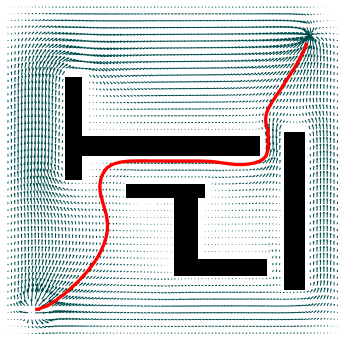
\includegraphics[width=0.9\linewidth]{figs/11/fig1}\caption{الخريطة الأولى}\label{11:fig:1}\end{subfigure}&
		\begin{subfigure}{0.4\textwidth}\centering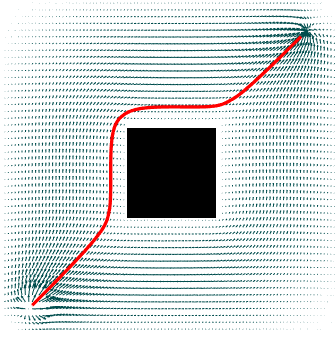
\includegraphics[width=0.9\linewidth]{figs/11/fig2}\caption{الخريطة الثانية}\label{11:fig:2}\end{subfigure}\\
		\newline
		\begin{subfigure}{0.4\textwidth}\centering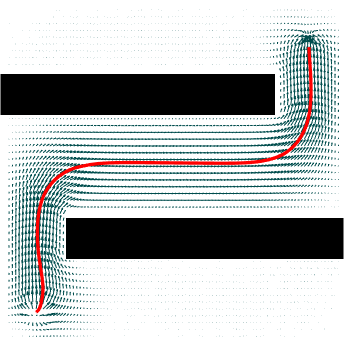
\includegraphics[width=0.9\linewidth]{figs/11/fig3}\caption{الخريطة الثالثة}\label{11:fig:3}\end{subfigure}&
		\begin{subfigure}{0.4\textwidth}\centering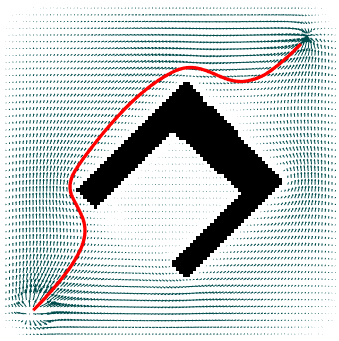
\includegraphics[width=0.9\linewidth]{figs/11/fig4}\caption{الخريطة الرابعة}\label{11:fig:4}\end{subfigure}\\
	\end{tabular}
	\caption{أداء الخوارزمية لعدة خرائط}
	\label{tab:mytable}
\end{table}
\end{center}


\subsection{الخوارزمية المقترحة للسرب}

أفضت الطريقة المتبعة في انتاج مسار لروبوت واحد في فضاء اختياري نتائج عالية الوثوقية والأمان، التجارب أثبتت بشكل كبير قدرة هذه الطريقة على إنتاج طريق ناعم حال وجود اتصال بين المبدأ والهدف. يعد تعميم هذه الطريقة لضمان وصول مجموعة روبوتات إلى هدفها عملية غاية في التعقيد، وذلك خصوصاً لطبيعة الروبوتات الغير هولنومية المدروسة في هذا المشروع. يمكن الاستدلال إلى تهجين بين عدة طرق لإيجاد ما يناسب حالات خاصة من فضاءات اعمل في الدراسات المرجعية.
لنتمكن من انتاج حل يتسم بالبساطة الاستدلالية وبالحتمية والكمالية، يجب العودة إلى الآلية التي تتصرف فيها جزيئات سائل وجدت نفسها في حقل كموني. إن ألية التفكير هذه تفضي إلى نوعين من الحلول:

\begin{itemize}
	\item الروبوتات غير واعية لبعضها
	\item الروبوتات (الجزيئات) واعية لبعضها
\end{itemize}

يمكن مقاربة الحل الأول بجزيئات سائل لا نيوتوني تسير في حقل السرعة المنتج، والطريقة الثانية بعدد من الأجسام صلبة تهوي في هذا الحقل.

\subsubsection{الروبوتات غير الواعية لوجود السرب}

هنا يتم احتساب حقل كموني صغير خارج من كل روبوت في السرب وإضافة هذه الحقول إلى حقل السرعة منهاً للتصادم، يتم هنا احتساب جميع قيم السرعة في كل نقاط الفضاء عن طريق أخذ جريان المائع من جهة والجيران من جهة أخرة. يمكن التحكم بقوة الحقل الكموني النافر الصادر عن كل روبوت بتغيير بارامترات الحساب.
ألية الحساب:

يتم أولاً ملء الخريطة فارغة بأجسام تتناسب أبعادها مع أبعاد الروبوتات الباقية في السرب، ثم يتم حساب تحويل المسافة للمصفوفة الناتجة \textenglish{(distance transform).} يتبع هذه الخطوة القيام بعملية مشروحة في الجدول \ref{11:fig:process}.





	\begin{table}
		\centering
		\begin{tabular}{cp{150pt}}
			\begin{subfigure}{0.35\textwidth}
				\centering
				\includesvg[width=0.9\linewidth]{figs/11/fig5}
			\end{subfigure}&  انشاء مصفوفة بأبعاد الخريطة ياوضع عليها الروبوتات الباقية من السرب. أبعاد الروبوتات في المصفوفة يتناسب مع أبعاد الروبوت (المصفوفة $\mathcal{M}$) \\
			\begin{subfigure}{0.35\textwidth}
				\centering
				\includesvg[width=0.9\linewidth]{figs/11/fig6}
			\end{subfigure}& التحويل المسافي $D(\mathcal{M})$\\
			\begin{subfigure}{0.35\textwidth}
				\centering
				\includesvg[width=0.9\linewidth]{figs/11/fig7}
			\end{subfigure}&  $\mathcal{M}_2 = \epsilon (1/D(\mathcal{M}) - 1/k )^2$ \\
			\begin{subfigure}{0.35\textwidth}
				\centering
				\includesvg[width=0.9\linewidth]{figs/11/fig8}
			\end{subfigure}& $ \mathcal{M}_2 > k $ \\
			\begin{subfigure}{0.35\textwidth}
				\centering
				\includesvg[width=0.9\linewidth]{figs/11/fig9}
			\end{subfigure}& $ \nabla (\mathcal{M}_2 > k) $
		\end{tabular}
		\caption{عملية حساب المسار في الحالة الأولى من الحل}
		\label{11:fig:process}
	\end{table}


ثم يتم جمع الحقل الناتج إلى حقول السرعة وإنتاج الحقل الخاص بكل روبوت. انزلاق الروبوت على الحقل الناتج يضمن وصوله إلى الهدف بسلاسة. انظر الشكل \ref{11:fig:square_map} كمثال.

\begin{figure}[htbp]
	\centering
	\includesvg[width=0.7\linewidth]{figs/11/square_map}
	\caption{مثال عن الطريقة المقترحة}
	\label{11:fig:square_map}
\end{figure}

\subsubsection{الروبوتات الواعية لوجود السرب}


يتم في هذه الطريقة برمجة وجود نابض ومخمد بين كل روبوتين متجاورين من روبوتات السرب. وجود هذه النظام الميكانيكي سيضمن حركة السرب ضمن تشكيلة معينة نجمية تحدد عناصرها من بارامترات البرمجة. يمكن حساب القوة المتبادلة بين روبوتين متجاورين كالتالي:

\begin{equation}
F_{ij}=F_k+F_c=k\left(d_{ij}-d_0\right)+c\frac{d}{dt}\left(d_{ij}-d_0\right)
\end{equation}
وبعدها يتم تحصيل القوى باستخدام:
\begin{equation}
\vec{\mathcal{F}_i}=\ \sum_{j\in\mathbb{N}_i}{\vec{F_{ij}}\ }
\end{equation}


تجمع القوة السابقة مع القوة الناتجة عن وجود حقل سرعة مائع لإنتاج خطوة المشي الجديدة. انظر الشكل \ref{11:fig:6}

\begin{figure}[htbp]
	\centering
	\includesvg[width=0.7\linewidth]{figs/11/fig61}
	\caption{القوى المتبادلة بين الروبوتات ممثلة كعناصر ميكانيكية}
	\label{11:fig:6}
\end{figure}


	
	\section{التغذية الراجعة لشعاع حالة الروبوتات}
	لإيجاد مواقع الروبوتات سوف يتم استخدام نظام التعريف ArUco، حيث تتم طباعة عدة QR codes ولصقها على سطح كل روبوت. بعد القيام بعملية معايرة لبارامترات الكاميرا الـIntrinsic والـExtrinsic يمكن أيجاد المصفوفة $ \mathbb{C} $ المستخدمة في \ref{eq:cameramatrix}.

\begin{equation}\label{eq:cameramatrix}
\mathbb{P}=\left(\begin{matrix}p_x\\p_y\\1\\\end{matrix}\right)=\mathbb{C}\times\left(\begin{matrix}r_x\\r_y\\r_z\\1\\\end{matrix}\right)=\mathbb{C}\times\mathbb{R}
\end{equation}
حيث يمثل $ \mathbb{P} $ موضع الروبوت في إحداثيات حساس الكاميرا، و$ \mathbb{R}  $إحداثيات الروبوت في الاحداثيات الأرضية، و$  \mathbb{C}  $ مصفوفة الكاميرا (Camera Matrix).


منها يمكن نقل كل بكسل من بكسلات الكاميرا الى الاحداثيات الأرضية باستخدام الـpseudo-inverse للمصفوفة $\mathbb{C}$. نذكر هنا أن المصفوفة $ \mathbb{C} $ :

\begin{equation}
\mathbb{C}=\mathbb{K}\times\left(\mathbb{R}\ |\ {T}\right)
\end{equation}

حيث تمثل المصفوفة $ \left(\mathbb{R}\ |\ {T}\right)  $ التحويل المتجانس الذي ينقل $ \mathbb{R}  $ الى احداثيات الكاميرا، والمصفوفة $ \mathbb{K}  $ تقاس من بارامترات العدسة والحساس وتشكّل كالتالي:
\begin{equation}
\mathbb{K}=\left(\begin{matrix}f_x&0&0\\s&f_y&0\\c_x&c_y&1\\\end{matrix}\right)
\end{equation}

يمثل كل من $ f_x, f_y $ البعد البؤري للعدسة، وs معامل انحراف الحساس، و $c_x, c_y$ يمثلان مركز الحساس بوحدات البكسل.
نذكر هنا أنه من الواجب القيام بعملية معايرة تسبق مرحلة نقل كل نقطة من نقاط الكاميرا الى الاحداثيات الواقعية وذلك لتقريب الكاميرا الموجودة أقرب ما يمكن الى نموذج الـ pinhole\ camera الموجود في المعادلات السابقة.



	
	\section{النموذج الرياضي العام للروبوت}
	
	النموذج الديناميكي للروبوت التفاضلي مدروس بشكل كامل مع استنتاجه في أغلب الكتب النصية الخاصة بأساسيات علم الروبوت. نكتفي هنا بإدراج معالة$  \dot{\mathbb{S}\ } $

\begin{equation}
\dot{\mathbb{S}}=\left(\begin{matrix}\dot{x}\\\dot{y}\\\dot{\theta}\\\end{matrix}\right)=\left(\begin{matrix}\frac{\left(u_1+u_2\right)}{2}\cos {\theta}\\\frac{\left(u_1+u_2\right)}{2}\sin{\theta}\\\frac{\left(u_1-u_2\right)}{l}\\\end{matrix}\right)
\end{equation}

حيث يمثل $ u_1 $, $ u_2 $ السرعة الخطية للعجلات، و$ l $ المسافة بين العجلتين.


	
	\section{دراسة العجلات}
	تخدم العجلات وظيفتين رئيسيتين: الأولى هي دورها الأساسي لتحريك الروبوت، والثانية هي كأقراص مشققة لتسجيل حركة المحركات. نناقش في هذا القسم الأدوات الرياضية والشروط التصميمية الموافقة لما سبق.
العجلات للحركة
عند اجراء التجارب المخبرية على سرعات المحركات الموجودة متبوعة بعلب سرعتها، وجدنا أن السرعة عند $ 7.5 V $ (أي السرعة الأعظمية) كانت $ 135 $ دورة في الدقيقة. عند وضع شرط أن الروبوت يجب أن يكون قادر على قطع الحلبة شاقولياً أو افقياً خلال مدة أقصاها عشر ثوان، وجدنا أن السرعة الخطية يجب أن تكون أكبر من $ 0.24\ m.s^{-1} $. هذا جعل من السهل حساب أن نصف قطر الدولاب المطلوب يجب أن يكون أكبر من $ 1.7E-2\ m.  $. ان اختيار نصف قطر الدولاب أيضاً يخضع أيضاً لقيد آخر هو شقوق مسجلات الحركة.



\subsubsection{العجلات كمسجلات حركة}

من المعلوم أنه لإنشاء نظام تحكم دقيق يجب وجود نظام تحسس للزاوية وسرعة حركة المحركات. أول طريقة وأكثرها شيوعاً هي استخدام قرص مشقق بفتحات ذات ابعاد متساوية. يقوم مقطع ضوئي بمقاطعة المتحكم عند تسجيل مرور فتحة أمامه مما يسمح للمتحكم بتسجيل عبور هذه الفتحة، مما يؤدي لتسجيل تغير في الزاوية مقداره الزاوية المصممة بين الفتحتين$  \vartheta $.

\begin{equation}
	\vartheta=\frac{2\pi}{n}
\end{equation}

حيث يمثل n عدد الفتحات الموجودة على القرص. نعرف $ \phi $ بأنها الزاوية التي يمسحها المقطع الضوئي لعبور شق واحد. ومنه يمكن تعريف $ \eta=\frac{\phi}{\vartheta}$ ، وهي نسبة عرض الشق الى مجمل الزاوية $ \vartheta $. يمكن مضاعفة الدقة عن طريق جعل وحدة المقاطعة الخارجية الموجودة في المتحكم AVR تقوم بتسجيل الحافة الصاعدة والهابطة في إشارة المقطع. فتصبح $  \Delta d $ (أصغر مسافة يمكن للمسجل قراءتها):

\begin{equation}
\Delta d=\frac{\vartheta}{2}r=\ \frac{\pi}{n}r
\end{equation}

يسمح وجود مقطع ضوئي واحد بتسجيل تغيرات الزاوية دون معرفة اتجاه الدوران. لقراءة اتجاه الدوران يجب إضافة مقطع ضوئي ثان متموضع مع فرق طور مقداره $ \vartheta/4  $ بالنسبة للمقطع الأول. ان تحريك المقطع الضوئي الثاني بعدد صحيح من مضاعفات $ \vartheta $ لن يغير من أداء عمله، لكن سيمكن المصمم من وضع كلا الحساسين في مكان مريح للفك والتركيب السريعين، مما يتوافق مع أحد أهم شروط الهيكل الخارجي للروبوت. نسمي المسافة بين الحساسين $  \psi $، ونعتبر أن الحساس الأول موضوع في المبدأ. 

بنقل هذه الشروط الى معادلات رياضية:

\begin{equation}
\vartheta=\frac{2\pi}{n}
\end{equation}

\begin{equation}
	\rightarrow\psi=\frac{\vartheta}{4}+{k}\vartheta=\left(\frac{\eta}{2}+{k}\right)\vartheta
\end{equation}

حيث $ {k}\in\mathbb{Z} $. إذا وضعنا شروط التالية:

\begin{itemize}
	\item دقة تسجيل الحركة يجب أن تكون أصغر من الدقة التي نستطيع الحصول عليها من الكاميرا.
	\item 	الزاوية بين المقطعين ($ \psi $) يجب أن تكون بين $ \frac{\pi}{4} $ و $ \frac{3\pi}{4} $.
	\item 	الزاوية بين المقطعين يجب أن تكون عدد صحيح من مضاعفات $ \frac{\pi}{180}\times5 $ لتسهيل عملية التصميم.
	\item 	عرض الشق لا يقل عن $1.2 E-3m$.
\end{itemize}

تولد الشروط مسألة البرمجة الصحيحة الآتية:

إيجاد $k, \eta, n, r$ حيث:
\begin{equation}
\psi=\frac{\phi}{2}+\mathcal{k}\vartheta=\left(\frac{\eta}{2}+\mathcal{k}\right)\vartheta
\end{equation}
\begin{equation}
\Delta d<2.5E-3\rightarrow\frac{r}{n}<2\times3.979E-4
\end{equation}
\begin{equation}
\psi=\mathcal{q}\ \left(\frac{\pi}{180}\times5\right),\ where\ \mathcal{q}\in\mathbb{Z}
\end{equation}
\begin{equation}
\frac{\pi}{4}\le\psi\le\frac{3\pi}{4}
\end{equation}


تسمى المسألة السابقة بأنها مسألة برمجة صحيحة بسبب وجود شرط انتماء $k$ الى مجموعة الأعداد الصحيحة. تم اثبات ان مسائل البرمجة الصحيحة هي مسائل NP-Hard ويحتاج حلها الى استخدام احدى تقنيات البحث مع القليل من الأمثلة. لن نتطرق الى استخدام هذه الطرق بسبب قلة عدد القيود على المسألة وصغر فضاء الحل، اذ يمكن عبور كل مجال الحل وتسجيل أفضل نقطة.


بعد حل المسألة السابقة يمكن استخلاص ما يلي:
\begin{equation}
\eta=0.5
\end{equation}
\begin{equation}
r=2E-2\ m
\end{equation}
\begin{equation}
\psi=210\times\frac{\pi}{180}\ rad
\end{equation}
\begin{equation}
n=33
\end{equation}
\begin{equation}
\Delta d=1.9E-3\ m
\end{equation}
ومنه ينتج تصميم العجل الموضح في الشّكل \ref{14:fig:1}.

\begin{figure}[htbp]
	\centering
	\includesvg[width=0.7\linewidth]{figs/14/fig1}
	\caption{تصميم عجلات الروبوت الناتج}
	\label{14:fig:1}
\end{figure}


	
	\chapter{بنية النظام الصلبة والبرمجية}
	
	\section{مقدمة}
	تتألف منصة العمل من: 1) فضاء عمل و2) الروبوتات. يشرح هذا الفصل الأسس الرياضية والمعايير المتبعة في تصميم ما سبق. نبدأ بشرح فضاء العمل والشروط التصميمية التي يفرضها على تصميم الروبوتات، ثم ننتقل الى عرض تصميم الروبوتات بشقيه الرياضي والحاسوبي.
	
	\section{فضاء العمل}
	يعرف فضاء عمل أي نظام روبوتي بمجموعة النقاط التي يستطيع الروبوت التواجد فيها بشكل آمن. نذكر هنا أن فضاء العمل لا يكون بالضرورة معرف بأساس الاحداثيات المكانية، على سبيل المثال، يمكن تعريف فضاء عمل ذراع روبوت بدلالة قيم مفاصل هذه الذراع، ويكون عدد أبعاده بعدد درجات حرية الذراع. يستخدم فضاء العمل بشكل أساسي للبحث عن مسارات يستطيع الروبوت عبورها بغية انجاز عمل معين. قد يكون هذا العمل غير مقيد، كإيجاد مسار بين موضع الروبوت الحالي ونقطة هدف محددة مسبقاً، وقد يكون مقيد بشروط معينة كإيجاد أقصر مسار أو أقلها استهلاكاً للطاقة. يمكّننا التعريف الجيد لفضاء العمل من إيجاد قيود المسألة التي يحاول الروبوت حلها بغية إيجاز المهمة الموكلة له، بمعنى أكثر دقة، تشكيل فضاء العمل هو أول خطوة من حل مسألة تخطيط المسار، التي تعتبر مسألة أمثلة.
يبين الشكل \ref{15:fig:4} فضاء عمل سرب الروبوتات. يتكون من مربع بضلع 2.4 متر وحواف مرتفعة. يحتوي المربع على عدة عوائق بأشكال مكعب أو أسطوانة وبأبعاد مختلفة. يمكن للعوائق أن تتحرك بالشكل المطلوب على الشبكة لتشكيل فضاء عمل ديناميكي.
 
 \begin{figure}[h]
 	\centering
 	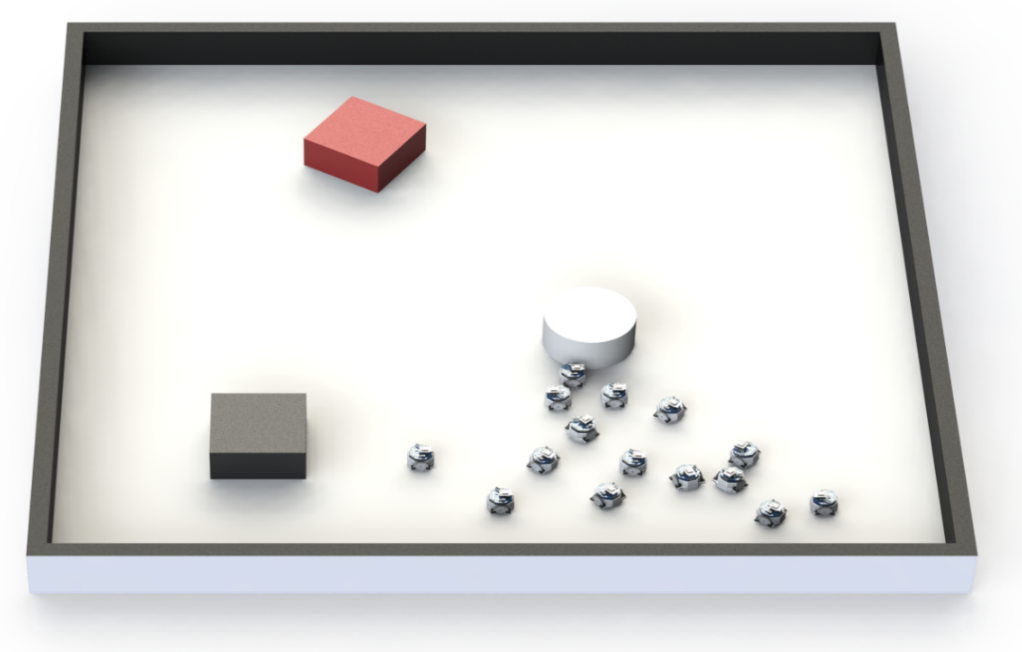
\includegraphics[width=0.8\linewidth]{figs/15/fig4}
 	\caption{ إخراج ثلاثي الأبعاد لمنصة العمل}
 	\label{15:fig:4}
 \end{figure}
	
	\section{بنية النظام الصلبة}
	\subsection{نظرة عامة}



\subsection{الأدوات}
\subsubsection{التغذية الراجعة}
إنّ تحديد نظام التّغذية الرّاجعة (XYTheta feedback) كان الخطوة الأساسيّة لنا لوضع تصوّر أساسي للمشروع ولبدء عمليّة التّصميم واختيار القطع الإلكترونيّة بحيث نحصل على أفضل أداء ممكن وفق تصميم مناسب وأسعار مقبولة. اعتمدنا في هذه المرحلة على نظام نقاط بين 1 و 5 - حيث يشير الرّقم 5 إلى الأفضليّة العليا – للمفاضلة بين الخيارات المتاحة وفق معايير محدّدة كما هو موضّح في الجدول أدناه.

\begin{table}[h]
	\begin{tabular}{lccccccc|}
		\cline{2-8}
	\multicolumn{1}{l|}{} & الحاجة للاختبار  &  فعالية التحكم & سهولة التطبيق & سهولة التصميم  & الحاجة  & السعر &    \\ \hline
		\multicolumn{1}{|l}{Dead Reckoner} & 3 & 4 & 4 & 5 & 3 & 5 & 24 \\ \hline
		\multicolumn{1}{|l}{Mouse Sensor}  & 1 & 5 & 2 & 3 & 5 & 4 & 20 \\ \hline
		\multicolumn{1}{|l}{Camera}        & 5 & 5 & 2 & 5 & 3 & 5 & 25 \\ \hline
	\end{tabular}
\end{table}


بعد عمليّة المقارنة وبناءً على النّتائج الموضّحة أعلاه كان خيار استخراج مواقع الرّوبوتات من كاميرا مثبّتة فوق حلبة عمل الرّوبوتات هو الخيار الأفضل. 
أمّا عمليّة اختيار الكاميرا فكانت ترتكز على معيارين أساسين وهما الحصول على تغطية كاملة للمنّصة و عدد الأطر التي يمكن الحصول عليها في الثّانية الواحدة. لذلك قمنا باختيار كاميرا ستريو واسعة الزّاوية الّتي تعدّ خياراً مناسبا لنا. حيث أنّ  أبعاد حساس كل كاميرا 960×2560 بكسل. يمكن بسهولة إيجاد أنّ أصغر مسافة يمكن قياسها باستخدام الكاميرا عن طريق تقسيم عرض فضاء العمل ( على دقة حسّاس الكاميرا و النتيجة هي 2.5 mm. بالإضافة إلى إمكانيّة الحصول على 16 إطار بالثّانية وهو تردّد كافٍ لمتابعة سير الروبوتات وتحديد مواقعها.

\subsubsection{المحرك}
المعايير الأساسيّة الّتي تمّ اعتمادها لاختيار المحركات: طريقة قياس لموضع وطريقة قيادة الرّوبوت ولقد اعتمدنا لتحديد ذلك النّظام النّقطي السّابق الّذي اعتمدناه لتحديد نظام التّغذية الرّاجعة في الفقرة السّابقة.

\begin{table}[h]
	\begin{tabular}{lccccccc|}
		\cline{2-8}
		\multicolumn{1}{l|}{} & الحاجة للاختبار  &  فعالية التحكم & سهولة التطبيق & سهولة التصميم  & الحاجة  & السعر &    \\ \hline
		\multicolumn{1}{|l}{ODD BLDC} & 1 & 5 & 1 & 1 & 3 & 4 & 15 \\ \hline
		\multicolumn{1}{|l}{Micro Servo}  & 5 & 3 & 5 & 5 & 3 & 1 & 22 \\ \hline
		\multicolumn{1}{|l}{Gear DC}        & 2 & 4 & 1 & 1 & 2 & 3 & 13 \\ \hline
	\end{tabular}
\end{table}


كما نرى في الجدول السّابق فإنّ محرّك الـ Micro servo كان الخيار الأكثر ملائمة ولاسيّما مع سهولة استخدامه وتغليفه الّذي سوف يسهّل عمليّة التّصميم بشكل كبير  بالإضافة إلى سعره المقبول. ولكنّه كان بحاجة لعمليّة اختبار للتأكد من مدى قدرتنا على التّحكم به و عن مدى قدرتنا على التّحكم به. لذلك قمنا باالتّجريب على محرك SG90 Continuous 360 Degree. يبلغ وزن المحرك 9 غرام وعزمه عند جهد تغذية 4.8 فولت $1.3 Kg.cm$ وسرعة الدوران الأعظمية 110 دورة في الدقيقة.

لكنّ نتائج الاختبار لم تكن مرضية بشكل كامل؛ حيث بينت الاختبارات وجود منطقة ميتة في خرج الاكودر الداخلي للمحرك dead band. لكنّ الخيارات الاخرى كانت غير مناسبة من ناحية التّوافر؛ لذلك لجأنا إلى حل آخر، وهو فصل محرّك التّيار المستمرّ الموجود داخل الـ SG90  عن دارة قيادته ووصله مع المقاومة المتغيّرة الدّاخلية إلى دراتنا السفليّة و باالتّالي يمكن استخدام محرّكات تيّار مستمرّ بحجم مناسب وضمن تغليف مناسب مّما سهّل علينا عمليّة تصميم الجسم وتصغير حجمه بالإضافة إلى السّعر المناسب. كما أنّنا سوف نقوم باستخدام العجلات كمسجلّات للحركة من أجل تحكّم أكثر دقّة.

\subsubsection*{قيادة المحرك}
 بالنّسبة لقيادة محركات التيار المستمر، فتم ذلك باستخدام الجسر L298. يعاني الجسر من عدة مشاكل أهمها قدم تكنولوجيا TTL المستخدمة في صناعته، وأيضاً كبر حجمه. ممّا فرض قيوداً في الحجم والشّكل على تصميم الدّارات  لذلك استخدمنا L298N - Dual Full-Bridge Driver IC وسنرى لاحقا كيف أنّ تصميم الدّارات وتجميعها مكّننا من تنفيذ الشروط المطلوبة للتّصميم ضمن القيود المفروضة عليه.
 
\subsection{وحدة التحكم}
لتغطية كافة احتياجات النظام الإلكتروني تمّ وضع عدة نقاط رئيسية يجب على النظام المدمج في الروبوت شملها:

\begin{itemize}
	\item اتصال آمن وبتأخير (latency) منخفضة بين الروبوت والنظام المركزي.
	\item القدرة على قيادة محركي DC بجهد أعظمي 7.5 v وتيار 0.5 A أعظمي.
	\item عرض نبضة بتردد متوافق من الثابت الزمني للمحرك.
	\item نظام تحديد سرعة وموضع كل من محركي التيار المستمر.
	\item نظام تغذية.
	\item وحدات ادخال وإخراج بدائية بغية الـdebugging وتبديل البارامترات الداخلية on-the-run.
\end{itemize}

اعتمدنا على سلسلة متحكمات الـ 8 bit الخاصة بشركة Atmel ذات الـInstruction set RISC. يوجد في هذه المتحكمات 35 تعليمة بالإضافة لعدة وحدات توقيت ومقاطعات داخلية وخارجية تجعل المهمة المطلوبة ممكنة. ولقد اخترنا المتحكّم  Atmega328p tqfp.

يمتلك المتحكم Atmega328p المواصفات الآتية:
\begin{english}
\begin{itemize}
	\item Two 8-bit Timer/Counter
	\item One 16-bit Timer/Counter
	\item UART Connection Unit
	\item Two External Interrupt Unit
	\item I2C Unit
	\item Three 8-bit I/O units
	\item One ADC Unit with MUX to 8-bit I/O Unit
\end{itemize}
\end{english}


يضمن وجود ثلاث مؤقتات/عدادات قدرة النظام على جدولة المهام حسب أولوياتها وحسب الوقت المطلوب لها. كما انها توفر العتاد المطلوب لتشكيل إشارة بعرض نبضة متغير PWM تستخدم لقيادة محركات التيار المستمر. (يتم تشكيلها باستخدام الـHardware). توفر وحدة الـUART الاتصال المباشر بين وحدة الاتصال وبين المتحكم وبشكل سهل ومباشر وآمن من الأخطاء. أما بالنسبة للمقاطعات الخارجية: فهي تسمح للمتحكم بتسجيل الحركة التي تسجلها المقاطعات الضوئية المستخدمة في قراءة دوران المحرك.

\subsection{التغذية}

باختلاف التّصورات المحتملة لسرب الرّوبوتات، فإنّ كل روبوت ضمن السّرب يحتاج إلى إمداده بطاقة لإكمال المهمّة الموكلة له. ولقد قمنا باختيار بطّاريات  Lithium-Ion القابلة لإعادة الشّحن؛ حيث يمكن إعادة شحن هذا النّوع من البّطاريات مئات المرّات مع الحفاظ على ثباتها وأدائها مقارنةً بغيرها من البطّاريات. تميل بطّاريات Lithium-Ion إلى أن تكون ذات كثافة طاقة أعلى، معدّل تفريغ ذاتي أقلّ من البطّاريات الأخرى القابلة لإعادة الشّحن؛ ممّا يؤدّي إلى تحسين كفاءة الطاقة حيث تتمتّع الخليّة الواحدة باحتفاظ بالشّحن لفترة أطول من أنواع البطّاريات الأخرى. أمّا بالنّسبة للشكل: فلقد اخترنا بطاريات بأبعاد ( 4 mm× 4 cm ×5 cm ) لكي تتناسب مع التّصميم. وتقدّم هذه البطّاريات جهداً مقداره 3.7 V وتتوضّع عليها دارة حماية.

إنّ استخدام مصدر تغذية قابل لإعادة الشّحن يفرض علينا استخدام وحدة شحن وتفريغ. ولقد استخدمنا وحدات TP4056A المستخدمة لشحن وتفريغ بطّاريات اللّيثوم أيّون. ونظراً إلى أنّ البطّاريّات المستخدمة تقدّم جهد 3.7 V؛ احتجنا إلى استخدام وحدة رافع جهد (DC- DC convertor). إنّ دخل دارة رافع الجهد يتراوح بين 3 إلى 15 فولت، بينما يكون الخرج من 4 إلى 35 فولت، ويتمّ ضبطها لإعطاء الخرج المطلوب بشكل يدوي.


\subsection{نظام الاتصال}
بعد قراءة الدّراسات المرجعيّة واستشارة المختصّين تم اعتماد تقنية الواي فاي لربط الروبوتات مع بعضها ومع الحاسوب المركزي. ولاختيار وحدة الواي فاي المناسبة.
% Please add the following required packages to your document preamble:
% \usepackage{multirow}
\begin{table}[h]
	\resizebox{\textwidth}{!}{\begin{tabular}{lrccccc|}
			\cline{3-7}
			\multicolumn{2}{l}{\multirow{2}{*}{}}                                                                                                               & \multicolumn{2}{|c|}{\textbf{وحدات   بدائية}}       & \multicolumn{3}{c|}{\textbf{وحدات   مطوّرة}}                                \\ \cline{3-7} 
			\multicolumn{2}{l}{}                                                                                                                                & \multicolumn{1}{|c}{ESP-01}              & ESP-12e             & NodeMcu-DevKit-V1.0 & NodeMcu-Lua-WIFI-Board & Wemos-D1-Mini       \\ \hline
			\multicolumn{1}{|l|}{المداخل   والمخارج للأغراض العامّة} & GPIO & 2                   & 11                  & 11                  & 11                     & 11                  \\ \hline
			\multicolumn{1}{|l|}{محوّل   تماثلي رقمي}                & ADC       & -                   & 1                   & 1                   & 1                      & 1                   \\ \hline
			\multicolumn{1}{|l|}{هوائي}                              & Antenna                                                                                  & مطبوعة   على الدارة & مطبوعة   على الدارة & مطبوعة   على الدارة & مطبوعة   على الدارة    & مطبوعة   على الدارة \\ \hline
			\multicolumn{1}{|l|}{إمكانيّة   الوصل المباشر}           & USB-to-Serial                                                                            & غير ممكن            & غير ممكن            & ممكن                & ممكن                   & ممكن                \\ \hline
			\multicolumn{1}{|l|}{عامل   الشّكل}                      & Form                                                                              & صغير                & متوسط               & كبير                & كبير                   & متوسط               \\ \hline
			\multicolumn{1}{|l|}{وحدة الـ  ESP8266}                  & ESP8266 Module                                                                           & -                   & -                   & ESP12E & ESP12E   & ESP12E       \\ \hline
			\multicolumn{1}{|l|}{شريحة   الوصل المباشر}              & Serial                                                                              & -                   & -                   & CH340G              & CP2102                 & CH340G              \\ \hline
			\multicolumn{1}{|l|}{غطاء لحجب   التّرددات الرّاديويّة}  & RF-shield                                                                             & لايوجد              & يوجد                & يوجد                & يوجد                   & يوجد                \\ \hline
	\end{tabular}}
	\label{table::rfmodule}
	\caption{جدول مقارنة بين وحدات الاتصال المختلفة}
\end{table}

وتم التقييم وفق معايير معينة وهي الوثوقية، الحجم، التوافرية، السعر، وامكانية الوصل المباشر (USB-to-Serial) . بناءً على هذه المعايير والجدول السّابق قمنا باختيار وحدة الاتّصال Wemos  ؛ حيث أنّها تحقق ذات وثثوقيّة عالية مقارنة بسعرها وحجمها مناسب بالإضافة إلى توافرها.

\subsection{الدارة الالكترونية المطبوعة PCB}

يتم قيادة محرك التيار المستمر باستخدام الجسر L298. يعاني الجسر من عدة مشاكل أهمها قدم تكنولوجيا TTL المستخدمة في صناعته، وأيضاً كبر حجمه. ممّا فرض قيوداً في الحجم والشّكل على تصميم الدّارات. سوف نعرض في الفقرتين التاليتين تجميعة الدارات التي مكنتنا من تنفيذ الشروط السابقة ضمن قيود الحجم والشكل المفروضة عليه. حيث سنقوم في القسم الأول بشرح عملية تصميم أمّا في القسم الثّاني سوف نقوم باستعراض عمليّة التّصنيع.

\subsubsection{التصميم باستخدام الحاسب}
لقد استخدمنا البرنامج التّصميمي Altium لتصميم الطّبقة العلويّة والسفليّة. حيث أن الطّبقة العلويّة تحتوي على وحدة الاتصال والمتحكّم الصغري ووحدات الادخال والإخراج، بينما يحتوي يضم القسم السّفلي جسر القيادة، وحدات التغذية وشحن المدخرة، ودارات المقطعات الضوئية. 

\subsubsection*{الطبقة العلوية:  طبقة المعالجة والإشارة}
 هذه الطبقة مسؤولة عن أي اجراء على الروبوت القيام به حسابياً أو لتلقي أوامر الحركة من حاسوب مركزي. تحوي الطبقة متحكمين اثنين: الأول بمعمارية RISC AVR 8 bit والثاني 32-bit. يوفر المعالج الأول الوسائل المنطقية والتوقيتية للتحكم بالمحركات بدقة وكذلك لإجراء حسابات المعادلات الفروقية بدور تقطيع بالغ الدقة، أي للقيادة منخفضة المستوى. أما المتحكم الثاني فيوفر آلية اتصال ببروتوكول Wi-Fi بين روبوتات السرب وبين القاعدة، وكذلك بعض الحسابات عالية المستوى كتقطيع المسار وموائمة التراسل بين الروبوت والحاسوب المركزي وملاحقة حركة الروبوت. يوجد المنتج النهائي للدارة في الشكل \ref{15:fig:1}
 
 \subsubsection*{الطبقة السفلية: طبقة التضخيم والإشارة}
 إن العزل الحاصل بين كل من التضخيم والاشارة يضمن إمكانية ملاحقة الأخطاء وعزل السبب ان كان كهربائي أو الكتروني-برمجي. تضمن هذه الطبقة تحسس ومراقبة كل من موضع وتيار المحركات باستخدام مفاهيم كهربائية بسيطة، وكذلك توفر إمكانية الربط الكهربائي بين كل من دارتي الشحن ورفع الجهد من جهة، وبين المدخرة من جهة ثانية.
 ان استخدام الجسر L298 لم يكن الخيار الأنسب كهربائياً، خصوصاً مع هذا الحمل المنخفض نسبياً. لكن عدم توفر بديل مناسب ضمن شروط الحجم الموضوعة مسبقاً جعله الخيار السليم. يوجد على الدارة أيضاً ديودات حماية كون المحرك المستخدم من النوع المستمر. لمراجعة الملفات التصميمية انظر الشكل \ref{15:fig:1}
 
 \begin{figure}[htbp]
 	\centering
 	\includesvg[width=0.85\linewidth]{figs/15/fig15_1}
 	\caption{التصميم باستخدام الحاسب لكل من الطبقتين العلوية والسفلية}
 	\label{15:fig:1}
 \end{figure}

\subsection{عملية تصنيع الدارات}

بعد عمليّة تصميم الدّارات انتقلنا إلى مرحلة التّصنيع، حيث أنّ كل طبقة (السفليّة والعلويّة) عبارة عن دارة ثنائيّة الجوانب أي كلّ أنّ منهما تتألّف من طبقتي نحاس مطليتين بمادة الفايبر غلاس (FR4)بسماكة$ 1.8 mm$.  ليأتي بعد ذلك غطاء اللّحام وهي الّتي تمنح الدّارة لونها الأرجوانيّ (أو أيّ لون آخر)، حيث يتمّ وضع هذه الطّبقة على طبقة النّحاس لعزل المسارات النّحاسيّة من الاتّصال الغير مقصود مع أيّ معدن أو لحام أو أطراف موصلة أخرى وهذه الطّبقة تساعد في وضع اللّحام في مكانه الصّحيح وتجنّب اللّحام الخاطئ ممّا سهّل عمليّة لحام القطع الإلكترونيّة السّطحيّة (SMD).  يلي طبقة غطاء اللّحام طبقة بيضاء من الحرير تدعى الشّاشة الحريريّة $ (Silk screen) $، وتستخدم هذه الطّبقة في إضافة الأحرف والرّموز والأرقام إلى ألواح الـ PCB ممّا يسهّل عمليّة تجميع المكوّنات على الألواح وفهمها بشكل أفضل.  يوضّح الشّكل أدناه الدّارات بعد عمليّة التّصنيع.

\begin{figure}[h]
	\centering
	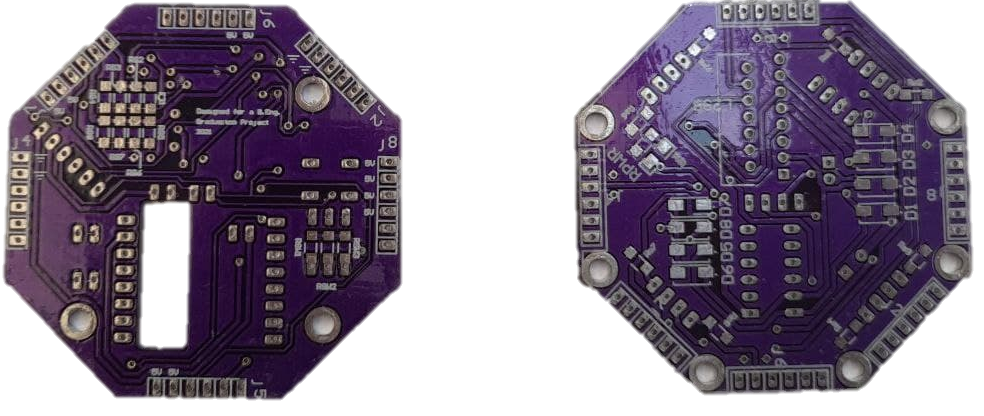
\includegraphics[width=0.9\linewidth]{figs/15/fig15_2}
	\caption{المنتج النهائي بعد تصنيع الدارة}
	\label{15:fig:2}
\end{figure}

\subsection{اختبار المنتج}

بعد عمليّة التّصنيع قمنا بعمليّة فحص للدّارات للتأكّد من التّوصيلات باستخدام الأدوات المختلفة. ووجدنا بعد عمليّة الفحص الأوليّة حدوث قصر في الدّارة ناتج عن انقطاع في الأرضي نتيجة القص الزّائد عند الأطراف، حيث أن أرضي الدّارة يتواجد في الأطراف والصّورة أدناه توضّح منطقة حدوث الانقطاع.

\begin{figure}[h]
	\centering
	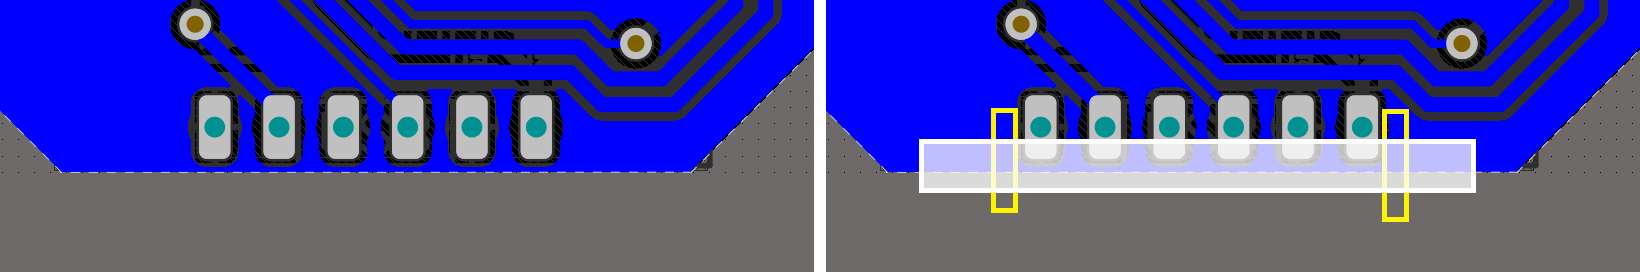
\includegraphics[width=0.9\linewidth]{figs/15/fig15_3}
	\caption{العطب الناتج عن التصنيع}
	\label{15:fig:3}
\end{figure}

لم يقتصر حدوث الانقطاع على منطقة الأرضي بل كان هناك انقطاعات في المناطق الموصلة عند الانتقال من جزء واسع إلى جزء ضيّق ($ necks $). بعد ذلك قمنا بإحصاء أماكن حدوث هذه المشكلة ووجدنا وجود انقطاعين في الطّبقة السّفليّة وانقطاعين في الطّبقة العليا وقمنا بوصل جميع المناطق المقطوعة بأسلاك خارجيّة.

\subsection{الجسم الخارجي والتحريك}

تم تصميم جسم الروبوت باستخدام برنامج SoildWorks واعتماد تصميم بسيط صغير الحجم بأبعاد 6×7×6 بشكل مثمن. تُثبت البطارية من الجهة السفلية للجسم ويوجد أماكن مخصصة لتثبيت المحركات والعجلات والمقاطعات الضوئية وتُبت الدراتين فوق الجسم باستخدام أربع براغي. كما هو موضح في الشكل 

 \begin{figure}[htbp]
	\centering
	\includesvg[width=0.85\linewidth]{figs/15/fig15_5}
	\caption{ الهيكل الخارجي للروبوت}
	\label{15:fig:5}
\end{figure}

تم تصنيع الجسم باستخدام تقنية الطباعة ثلاثية الأبعاد من مادة  Polylactic Acid (PLA)مع خصائص طباعة تتلخص في ارتفاع الطبقة 0.16 ملم وسماكة الجدران 0.8 ملم. 
بعد تجريب ثلاث ورشات متوفرة وسهلة الوصول جغرافيا، توصلنا إلى أفضل طباعة بشكل يضمن الجودة المطلوبة ولاسيما في تصنيع العجلات حيث أن أي اختلاف أو عدم انتظام في الثقوب سيؤثر مباشرة على قيم التغذية الراجعة التي سيعتمدها الروبوت لتتبع المسار الناتج. توضح الصورة \ref{15:fig:6} مقارنة بين علجة مثالية وعجلة ذات جودة تصنيع منخفضة.


\begin{figure}[h]
	\centering
	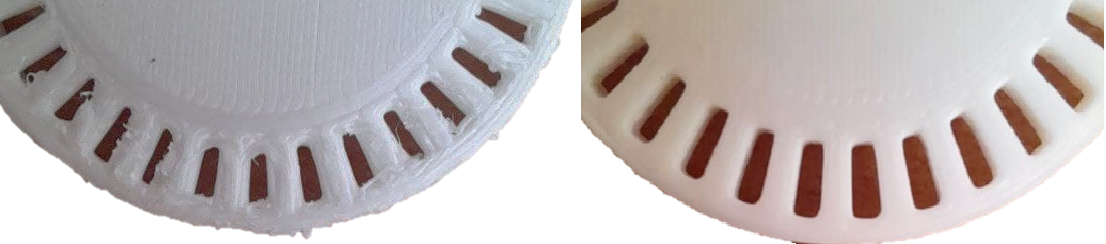
\includegraphics[width=0.9\linewidth]{figs/15/fig15_6}
	\caption{ مثال يوضح مقارنة بين سوء وجودة تصنيع العجلات}
	\label{15:fig:6}
\end{figure}



لضمان حركة مستقرة للروبوت على الأرض ونظراً لخفة وزن الروبوت، قمنا باختيار مادة مناسبة من الكاوتشوك لإحاطة إطارات كل العجلات و زيادة الاحتكاك وبعد التجريب تم تحقيق الغاية المرجوة حيث أن انزلاق العجلات على الأرض كان شبه معدوم. سنعرض النتائج النهائية لتركيب الروبوتات في فصل النتائج.

بالنّسبة لدور العجلات كمسجّلات حركة فكان يجب اختبار دقّة الطّباعة ثلاثيّة الأبعاد في إخراج الشّقوق الموجودة على العجلات، ولاختبار ذلك قمنا بتحريك العجلات بأقصى سرعة يمكن للروبوت السّير بها فكانت استجابة المقاطعات الضّوئيّة لعبور الشقوق عبرها كالتالي (الشكل \ref{15:fig:enc}): 


 \begin{figure}[htbp]
	\centering
	\includesvg[width=0.85\linewidth]{figs/15/fig_enc}
	\caption{استجابة المقاطعات الضّوئيّة}
	\label{15:fig:enc}
\end{figure}

\begin{figure}
	\centering
	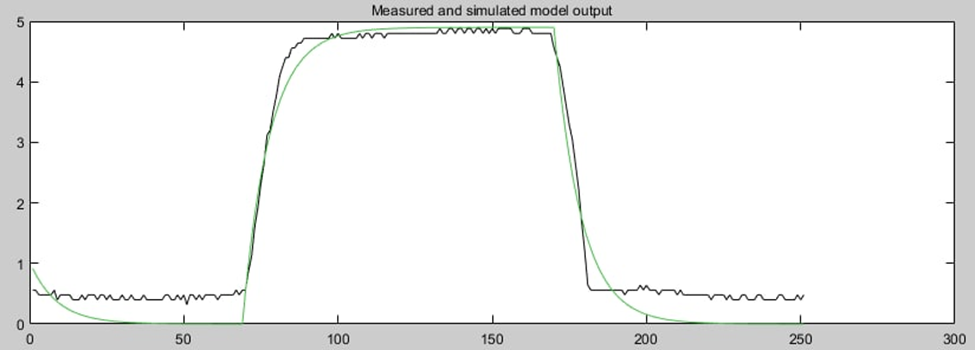
\includegraphics[width=0.9\linewidth]{figs/15/fig15_enc2}
	\caption{التقريب إلى نظام درجة أولى}
	\label{fig:fig15enc2}
\end{figure}

أمّا الخطوة التّالية فكانت اختبار استجابة الـ AVR للمقاطعات الضّوئيّة، وكما نلاحظ من قراءة الاستجابة الموضّحة في الشّكل \ref{fig:fig15enc3} وجود تاخير بسيط في استجابة الـ AVR.

\begin{figure}
	\centering
	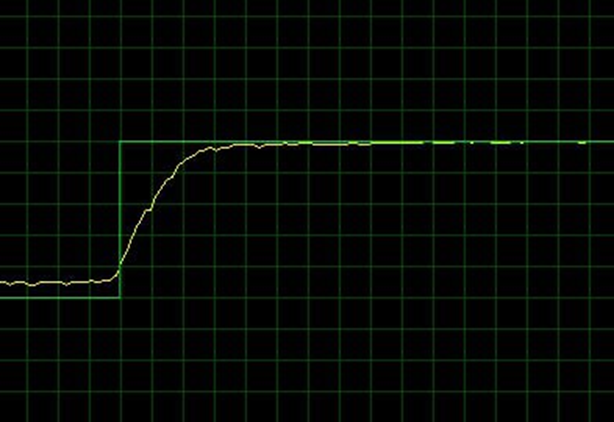
\includegraphics[width=0.7\linewidth]{figs/15/fig15_enc3}
	\caption{محاكاةاستجابة الـ AVR للمقاطعة الضّوئيّة}
	\label{fig:fig15enc3}
\end{figure}

ولتحسين قراءة المقاطعات الضّوئيّة قمنا بتصميم encoder وتصنيعه للحصول على حواف شقوق حادّة ومن ثمّ إطباقه على شقوق العجلات للحصول على أفضل استجابة ممكنة.

\begin{figure}
	\centering
	
\includegraphics[width=0.5\linewidth]{figs/15/fig15_enc4}
	\caption{طبقة بلاستيكية لتحسن قراءة المقطعات}
	\label{fig:fig15enc4}
\end{figure}

	\subsection{نظام الاتصال}
\subsubsection{طوبولوجيا الشبكة}
على مستوى طبقة الـ Data Link، فلدينا العديد من الخيارات المُتاحة. قمنا في البداية بالعمل على بروتوكول ESP-NOW المُطوّر من قبل Espressif، وإنّ الاتّصال اعتماداً على هذا البروتوكول هو اتّصال موثوق TCP من دون الحاجة إلى عمليّات المُصافحة.
نظراً لأهميّة موثوقيّة الاتّصال فقد قمنا باختبار البروتوكول ESP-NOW (one to many) على خمس عقد، حيث تكون أحد العقد هي الـ Master والبقيّة Slaves كما هو موضّح في الشّكل \ref{fig:fig161}.
\begin{figure}
	\centering
	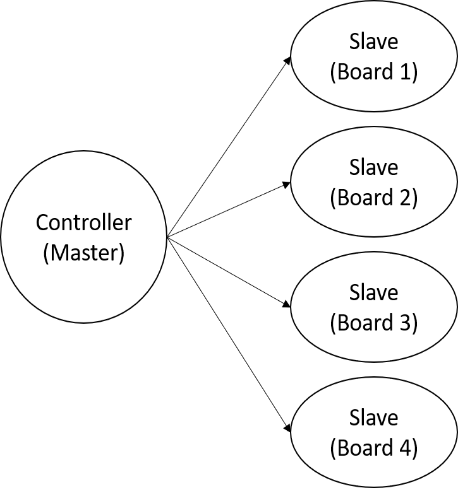
\includegraphics[width=0.4\linewidth]{figs/16/fig16_1}
	\caption{}
	\label{fig:fig161}
\end{figure}


يث قمنا في البداية بتعريف عنوان الـ MAC الخاص بكلّ شريحة اتّصال، ومن ثمّ إرسال إحداثيين x و y مولّدين عشوائياً لجميع العقد ألف مرّة وإعادة التّجربة من أجل أزمنة تأخير مُختلفة كما هو موضّح في الشّكل \ref{fig:fig162}، حيث يمثّل المحور الأفقي أزمن التأخير من أجل الشّرائح  الأربعة، أمّا المحور الشّاقولي فهو عبارة عن الرّسائل الألف المرسلة مُرتّبة من الرسالة الأولى في الأسفل إلى الرسالة الأخيرة في الأعلى.  يُعبّر اللّون الأحمر عن وصول الرّسالة فيما يشير الأسود إلى فشل تسليم الرّسالة.

\begin{figure}
	\centering
	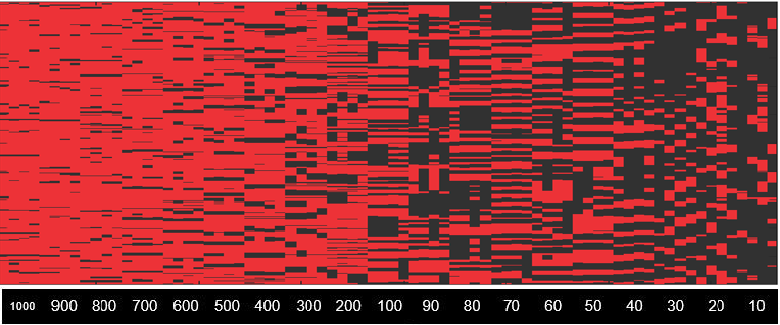
\includegraphics[width=0.9\linewidth]{figs/16/fig16_2}
	\caption{}
	\label{fig:fig162}
\end{figure}

\subsection{بروتوكول $ MQTT $}

هو بروتوكول نقل رسائل بين مخدّم زبون Client/Server بنمط نشر/اشتراك publish/subscribe قائم على الموضوع (Topic)؛ لأنّها ذات تطبيق مستقرّ للـ ESP8266  (باستخدام مخدّم Mosquitto MQTT) حسب [18]. وهنا يجب التّنويه لوجود ثلاث أنماط أساسيّة الاشتراك: النمط القائم على الموضوع والنمط القائم على المحتوى والنمط القائم على النوع.

إنّ بروتوكول MQTT (الموضح في الشكل \ref{fig:fig163}) يتكوّن من ثلاث أجزاء أساسيّة: المخدّم، النّاشر، والمشترك. يُعدّ المخدّم مسؤولاً عن إدارة شبكة من العملاء والّذين هم عبارة عن مزيج من النّاشرين والمشتركين؛ حيث أن النّاشر هو الجهاز الّذي يقوم بإرسال الرّسائل إلى المخدّم بحيث تكون هذه الرّسائل معنونة بعنوان موضوع (topic) بينما المشترك هو الجهاز الّذي يستمع لموضوع أو مواضيع معيّنة. يُمكن تشبيه الموضوع بوسم خاصّ بكلّ رسالة، ويمكن أن يكون وحيد الطّبقة أو متعدّد الطّبقات ويسمح هذا بتقسيم منطقي جيّد للمعطيات. على كلّ جهاز يرغب باستقبال موضوع معين أن يشترك به وذلك بإخبار المخدّم.
\begin{figure}
	\centering
	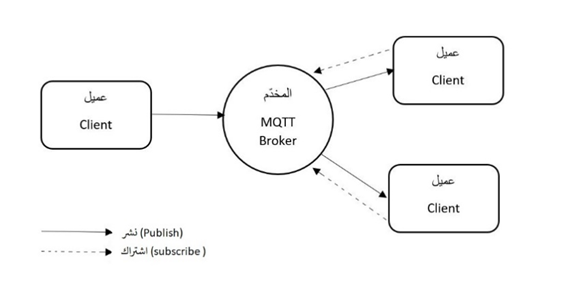
\includegraphics[width=0.7\linewidth]{figs/16/fig16_3}
	\caption{شكل توضيحي للأجزاء الأساسيّة في بروتوكول نقل الرّسائل MQTT}
	\label{fig:fig163}
\end{figure}

ليس هناك اتّصال مباشر بين المشترك والنّاشر وإنّما وببساطة يقوم المشترك بإخبار المخدّم أنّه مهتمّ بمواضيع محدّدة وبعد ذلك يقوم المخدّم بإرسال الرّسائل إلى المشتركين عند توافرها. إنّ نمط نشر/اشتراك مختلف تماماً عن نمط طلب/ردّ (request/response) المتّبع في بروتوكول الـ HTTP. كما أنّ بروتوكول الـ MQTT يعمل بالاعتماد على TCP/IP وعلى خلاف الـ HTTP فهو بروتوكول Binary وليس ASCII، وهذه إحدى ميّزاته فكما نعلم أنّ بروتوكولات الـ binary تستهلك كميّة نقل بيانات أقلّ من الشّبكة. بالإضافة إلى ذلك فهناك خيارات في بروتكول الـ MQTT تتعلّق بتوصيل الرّسالة بين المخدّم والعميل يُطلق عليها QoS (Quality of Service)، وهناك ثلاث خيارات بخصوص هذا الشّأن:

\begin{itemize}
	\item مستوى 0 (QoS = 0): توصيل الرّسالة مرّة واحدة في أفضل حالة؛ أيّ أنّه في حال لم يستلم المشترك الرّسالة فإنّ المُخدّم لن يقوم بإرسالها مرّة أخرى حيث لا يتوقّع المخدّم من المشترك تأكيد وصول الرّسالة (Acknowledgment).
	
	\item مستوى 1 (QoS = 1): توصيل الرّسالة مرّة واحد على الأقلّ. هذا يعني أنّ المخدّم يستمرّ بإرسال الرّسالة إلى أن يقوم المشترك باستلام الرّسالة ويرسل تأكيد باستلامها، وهذا يؤدّي إلى إمكانية وصول أكثر من رسالة واحدة إلى نفس المشترك.
	
	\item مستوى 2 (QoS=2): توصيل الرّسالة مرّة واحدة لزوماً، وهذا يعني أنّ الرّسالة يجب أن تصل لمرّة واحدة ودون تكرار المشترك.
	
\end{itemize}

وفي حال عدم اتّصال المشترك أساساً فيمكننا ضبط الإعدادات بحيث يبدأ الاتّصال بجلسة اتّصال نظيفة؛ حيث يقوم المُخدّم بتجاهل الرّسائل القديمة ويبدأ جلسة جديدة. بينما في حال تعطيل هذه الخاصيّة فإنّ الرسائل (من المستويين 0 و1) الّتي تمّ إرسالها إلى أحد المشتركين أثناء انقطاعه عن الشّبكة سوف تتراكم وسيقوم المُخدّم بإرسالها له فور اتّصاله بالشّبكة.
	\section{بنية النظام البرمجية}
	
	\subsection{نظرة عامة}
	كما أشرنا سابقاً فإنّ عمليّة التّحكم مركزيّة؛ حيث يوجد نظام تشغيل ROS على الحاسوب المركزي. يوجد على نظام ROS ثلاث عقد أساسيّة.
العقدة الأولى : تتصل مع الكاميرا المثبّتة أعلى المنصّة، حيث تقوم الكاميرا بإرسال الأطر لها لتقوم باستخلاص معلومات عن الخريطة ومواقع الرّوبوتات. ولتحقيق القراءة الدقيقة لمواقع الروبوتات في الزمن الحقيقي على الحاسوب المركزي سنعتمد مكتبة ArUco وهي مكتبة تستخدم في تطبيقات الواقع المعزز وتعتمد على مكتبة OpenCV  وتساعد في عملية معايرة الكاميرا. سيتم تثبيت علامات QR-markers على الروبوتات ومنه تقوم عقدة ال ArUCo في ال ROS تقوم باكتشاف وتحديد موقع العلامات وترسلها لل ROS-TOPIC .



\begin{figure}
	\centering
	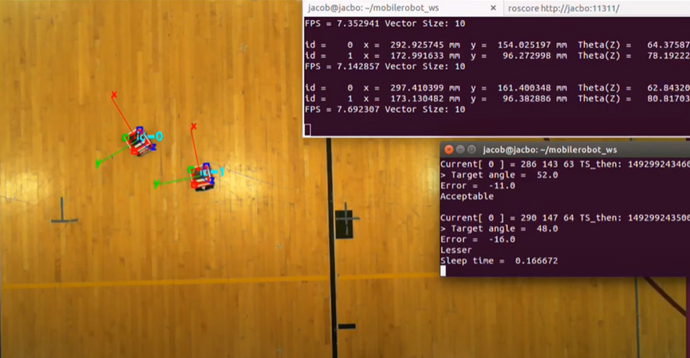
\includegraphics[width=0.7\linewidth]{figs/20/fig20_1}
	\caption{صورة توضيحيّة لآليّة عمل محددات ArUco}
	\label{20:fig:1}
\end{figure}

العقدة الثّانية: تقوم هذه العقدة باستقبال إحداثيّات الرّوبوتات والعوائق من العقدة الأولى عن طريق اشتراكها بالـ ROS TOPIC ذاته. بعد ذلك تتمّ على هذه العقدة عمليّة توليد المسار الأمثل وفق الخوارزميّة المختارة وإرسال نقاط المسارات الكاملة لجميع الرّوبوتات إلى العقدة الثّالقة.
العقدة الثّالثة: بعد استقبال هذه العقدة لنقاط المسارات الكاملة لجميع الرّوبوتات، تقوم بإرسال كلّ مسار إلى الـ Topic الخاص به  (إلى الرّوبوت الخاص به المشترك بنفس الـ Topic) عن طريق مخدّم الـ mqtt، لتكون هذه العقدة يمثابة عقدة وصل بين نظام ROS و مخدّم بروتوكول الـ mqtt.
وبعد أن يستقبل كلّ روبوت الرّسائل الخاصّة به تتكرّر هذه العمليّة بشكل دوري، ثمّ يقوم كلّ روبوت بتتيّع المسار وفق خوارزميّة تصحيح PID.

	
	\subsection{البنية البرمجية للروبوت منخفضة المستوى}
	كُتب برنامج تشغيل الروبوت باستخدام لغة c لقربها من العتاد الصلب ولدعمها من قبل منظومة GCC. كون المعالج بمعمارية 8 بت، هناك العديد من القيود على سرعة تنفيذ العمليات الحسابية عليه، فكلفة حساب متحول صحيح 32 بت أضعاف كلفة حساب ذات الرقم اذا كان مخزناً في متحول 8 بت. لا تواجه المعالجات الحاسوبية ذات معمارية 64 بت هذه المشاكل بشكل عام.

يمكن القول بأن نقطة الضعف الرئيسية لهذه المعالجات تكمن في عرض مسجلاتهاـ حيث تتميز بطيف واسع من المزايا المناسبة بشكل مطلق للتطبيق الحالي. 


صمم نظام تشغيل الروبوت بطريقة البرمجة التابعية لخلو لغة c من الأغراض والصفوف. نجد في الملحق توصيف شامل لكل أجزاء الكود البرمجي.

يتبع الروبوت المسار الواصل إليه عن طريق مصحح متقطع PID. تتكون حلقة الحساب من مصححين: الأول يتحكم بسرعة المحركين لعدم المسافة بين مركز الروبوت والنقطة الهدف، والثاني يقوم بعدم الزاوية بي شعاع سرعة الروبوت والشعاع الواصل بين مركز الروبوت والنقطة الهدف. عمل هذين المصححين ينتج مسارات مناسبة بين النقاط المتتابعة.


	
	
	\chapter{النتائج}
	
	بعد برمجة كل طرق توليد المسار المذكورة في الملف سيتم إجراء ما تبقى من تجارب تفريقية خلال الاسبوع القادم، حسث يجب إجراء جميع التجارب في ظروف عمل أقرب إلى المثالية وتضمن التطابق بين التكرارات. 
	
	يتم حاليا تحضير النتائج لكتابة الدرستين التاليتين:
	
	\begin{itemize}
		\item الدراسة الأولى عن تصميم وتنفيذ منصة سرب روبوتات لأغراض بحثية
		\item الدراسة الثانية عن مقارنة بين طريقة تخطيط المسار المقترحة والطرق الشهيرة في الدراسات المرجعية باستخدام المنصة المنجزة
	\end{itemize}
	
	
	\bibliographystyle{vancouver}
	\begin{english}
		\bibliography{ref}
	\end{english}
	
	\listoffigures
	\listoftables
	\chapter{الملحقات}
	\section{AVR C Code Referece Manual}
	
	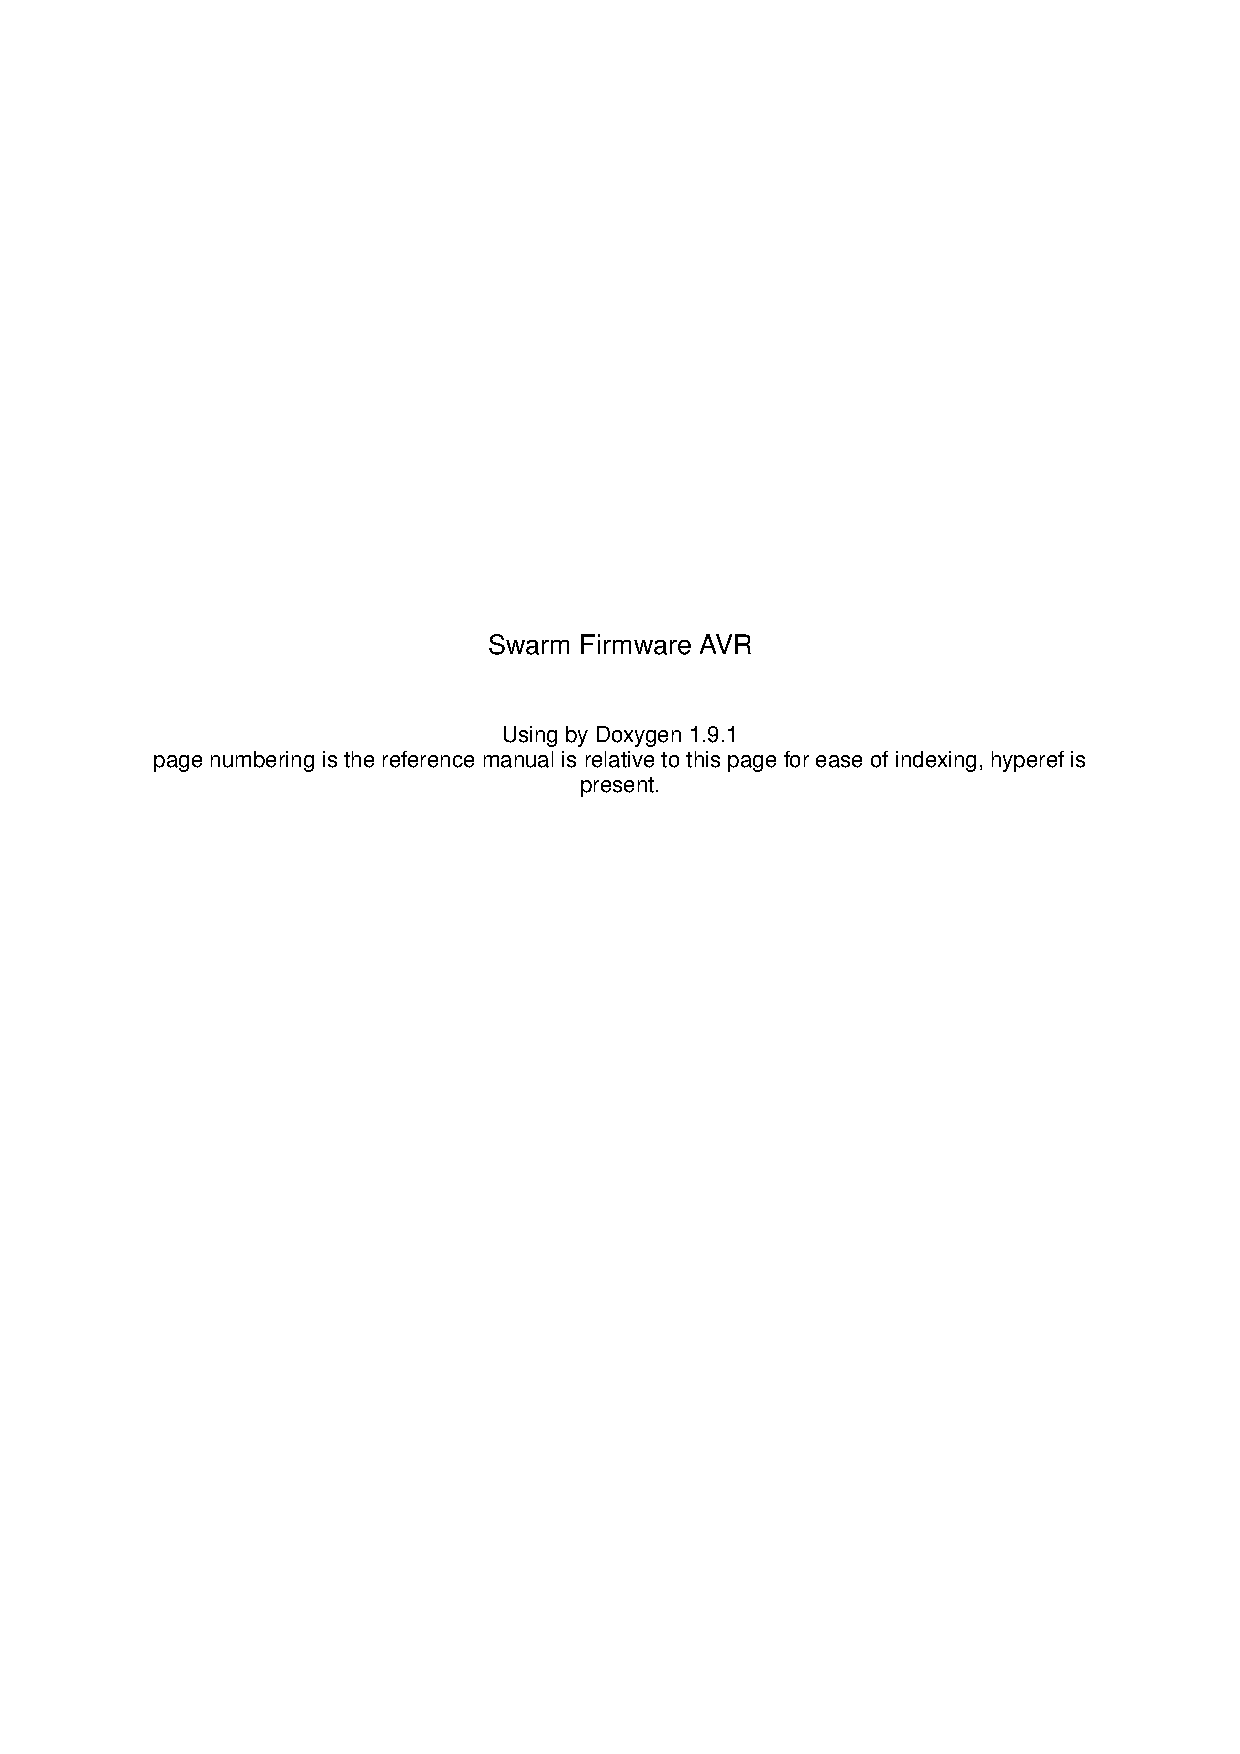
\includepdf[pages=-]{avr/refman.pdf}
	
\end{document}